% Master report
%
% Dates : 
%   - Submission :          01/09/2012
%
%
%
%\documentclass{llncs}
%
%\usepackage{graphicx}
%\usepackage{url}
%\usepackage{alltt}
%\usepackage{latexsym}
%%\usepackage{hyperref}
%%\usepackage{pslatex}
%%\usepackage{fullpage}
%%\usepackage{wrapfig}
%%\usepackage{floatfig}
%%\usepackage{multirow}
%\usepackage[usenames]{color}
%\definecolor{violet}{rgb}{0.5,0,0.5}
%\definecolor{gris25}{gray}{0.75}
%\definecolor{rose}{rgb}{1,0,1}
%\definecolor{bordeaux}{rgb}{0.6,0,0.2}
%\definecolor{turquoise}{rgb}{0.2,1,1}
%\definecolor{ciel}{rgb}{0.4,0.6,0.8}
%\definecolor{mer}{rgb}{0,0,0.4}
%\definecolor{orange}{rgb}{1,0.8,0}
%\definecolor{vertfonce}{rgb}{0,0.4,0.2}
%\definecolor{violetpastel}{rgb}{0.8,0.6,1}
%
%%\usepackage[ruled,vlined]{algorithm2e}
%%\usepackage{algorithm}
%%\usepackage{algpseudocode}
%
%\newtheorem{algor}{\noindent {\sc Algorithm }}
%\newenvironment{algorithm}{\begin{algor} \sl }{ \end{algor} } 
%\def\betab{\vspace{-0.10in}\begin{tabbing} 
%xxxxx\=xxxx\=xxxx\=xxxx\=xxxx\=xxxx\=xxxx\=xxxx\=xxxx\= \kill} 
%\def\entab{\end{tabbing}\vspace{-0.12in}}
%
%\usepackage{subfigure}
%\usepackage{multicol}
%\usepackage{amsmath}
%\usepackage{amssymb}
%
%\newcommand{\intervalle}[1]{{\llbracket {#1} \rrbracket}}

%\newenvironment{remarque}
%{\description \item[Remark:] \ \slshape}
%{\enddescription}
%
%

%
%
%\begin{document}
%
%%\pagestyle{headings} 
%%\mainmatter              % start of the contributions
%%
%\title{Enabling Partial Pivoting in Task Flow LU Factorization}
%%
%%%\titlerunning{Head Title}  % abbreviated title (for running head)
%%                                     also used for the TOC unless
%%                                     \toctitle is used
%%
%\author{ Omar Zenati\inst{1,2} \and Aurelien Bouteiller\inst{1} \and Emmanuel Agullo\inst{2} \and George Bosilca\inst{1} \and Mathieu Faverge\inst{1} \and Pierre Ramet\inst{2} \and Jack Dongarra\inst{1}}
%%% ~\footnote{This work is
%%%     supported by the ANR projects SOLTICE and NUMASIS
%%%     (http://solstice.gforge.inria.fr/ and
%%%     http://numasis.gforge.inria.fr/)}}
%%
%%
%%%%% modified list of authors for the TOC (add the affiliations)
%%\tocauthor{ TocAuthors }
%%
%\institute{
%  Innovative Computing Laboratory \\
%  The University of Tennessee, 1122 Volunteer Blvd., 37996, Knoxville, TN \\
%  \{bosilca,bouteill,dongarra,faverge\}@eecs.utk.edu
%\and
%  INRIA Bordeaux Sud-Ouest and LaBRI UMR 5800 \\
%  Universit\'e Bordeaux 1, 33405 Talence Cedex, France \\
%  \{ramet\}@labri.fr
%}
%
%\maketitle 
\documentclass[12pt]{report}
\usepackage{etex} 
\usepackage{lmodern}
\usepackage[a4paper]{geometry}
\usepackage[T1]{fontenc}
\usepackage[utf8]{inputenc}
\usepackage{moreverb}
\usepackage{amsmath}
\usepackage{amsfonts}
\usepackage{amssymb}
\usepackage{textcomp}
\usepackage{pifont}
\usepackage{geometry}
\usepackage[pdftex]{graphicx}
\usepackage{graphics}
\usepackage{url}
\usepackage{xspace}
\usepackage{graphicx}
\usepackage{float}
\usepackage[nottoc, notlof, notlot]{tocbibind}
\usepackage{pdfpages}
\usepackage{hyperref}
\hypersetup{
linkcolor= blue, 
colorlinks=true,
hyperindex=true,
breaklinks=true,
bookmarks=true,
urlcolor= black
}
\usepackage{listings}
\usepackage{latexsym}
\usepackage{color}
\usepackage{chngcntr}
\usepackage{stmaryrd}

%\renewcommand{\contentsname}{Plan}

\newtheorem{remarque}{Remarque}
\newtheorem{exemple}{Exemple}

\lstnewenvironment{code}[1][]{\lstset{
	numbers=left,
        numberstyle=\tiny,
	tabsize=8,
	language=matlab,
        basicstyle=\scriptsize,
        %upquote=true,
        aboveskip={1.5\baselineskip},
        columns=fixed,
        showstringspaces=false,
        extendedchars=true,
        breaklines=true,
        prebreak = \raisebox{0ex}[0ex][0ex]{\ensuremath{\hookleftarrow}},
        showtabs=false,
        showspaces=false,
        showstringspaces=false,
        identifierstyle=\ttfamily,
        keywordstyle=\color[rgb]{0.5,0,0.5},
        commentstyle=\color[rgb]{0.133,0.545,0.133},
        stringstyle=\color[rgb]{0.627,0.126,0.941},
	language=C,
        title=#1,
        frame=tlbr,
        frameround=tfff
}}{}


%%%%%%%%%%%%%%%%%%%%%%%%%%%%%%%%%%%%%%%%%%%%%%%% page de garde%%%%%%%%%%%%%%%%%%%%%%
\makeatletter
\def\clap#1{\hbox to 0pt{\hss #1\hss}}%
\def\ligne#1{%
\hbox to \hsize{%
\vbox{\centering #1}}}%
\def\haut#1#2#3{%
\hbox to \hsize{%
\rlap{\vtop{\raggedright #1}}%
\hss
\clap{\vtop{\centering #2}}%
\hss
\llap{\vtop{\raggedleft #3}}}}%
\def\bas#1#2#3{%
\hbox to \hsize{%
\rlap{\vbox{\raggedright #1}}%
\hss
\clap{\vbox{\centering #2}}%
\hss
\llap{\vbox{\raggedleft #3}}}}%
\def\maketitle{%
\thispagestyle{empty}\vbox to \vsize{%
\haut{}{}{}
\vfill
\vspace{2cm}
\begin{flushleft}
\usefont{OT1}{ptm}{m}{n}
\huge \@title
\end{flushleft}
\par
\hrule height 4pt
\par
\begin{flushright}
\usefont{OT1}{phv}{m}{n}
\Large \@author
\par
\end{flushright}
\vspace{1cm}
\vfill
\vfill
\bas{}{\@blurb}{}
\begin{center}
\@location \@date
\end{center}
}%
\cleardoublepage
}
\def\date#1{\def\@date{#1}}
\def\author#1{\def\@author{#1}}
\def\title#1{\def\@title{#1}}
\def\location#1{\def\@location{#1}}
\def\blurb#1{\def\@blurb{#1}}
\date{\today}
\author{}
\title{}
\location{Bordeaux}\blurb{}
\makeatother
\title{\texttt{Enabling Partial Pivoting in Task Flow LU Factorization}}
\author{Omar \textsc{Zenati}}
\location{Bordeaux }
\blurb{%
ENSEIRB-MATMECA\\
Computer Science Department\\
\textbf{Internship Report}\\[1em]
Tutors : Pierre \textsc{Ramet} \& George \textsc{Bosilca}\\
%Tuteur universitaire : Myriam \textsc{Desainte-Catherine}
}% 
%%%%%%%%%%%%%%% fin page de garde%%%%%%%%%%%%%%%%%
\makeatletter
\def\thickhrulefill{\leavevmode \leaders
\hrule height 1ex \hfill \kern \z@}
\def\@makechapterhead#1{%
\vspace*{10\p@}%
{\parindent \z@
{\reset@font
\usefont{OT1}{phv}{m}{n}
\LARGE Chapter \thechapter\par\nobreak}%
\par\nobreak
\vspace*{30\p@}
\interlinepenalty\@M
\usefont{OT1}{ptm}{b}{n}
{\raggedright \Huge \bfseries #1}%
\par\nobreak
\vskip 20\p@
\hrule height 2pt
\par\nobreak
\vskip 45\p@
}}
\def\@makeschapterhead#1{%
\vspace*{10\p@}%
{\parindent \z@
{\raggedleft \reset@font
\scshape \vphantom{\@chapapp{} \thechapter}
\par\nobreak}%
\par\nobreak
\vspace*{30\p@}
\interlinepenalty\@M
\usefont{OT1}{ptm}{b}{n}
{\raggedright \Huge \bfseries #1}%
\par\nobreak
\par\nobreak
\vskip 45\p@
}}
%%%%%%%%%%%%%%%%%%%%%%%%%%%%%%%%%%%%%%% fin titre%%%%%%%%%%%%%%%%%%%%%%

\newcommand{\dague}[0]{\textsf{DAGuE}\xspace}


\newcounter{taskflow_cnt}
\setcounter{taskflow_cnt}{0}
\newcounter{tmp_cnt}

\newenvironment{taskflow}{%
\renewcommand{\figurename}{Task flow}
\renewcommand{\thefigure}{\arabic{figure}}
%\counterwithout{taskflow_cnt}{chapter}

\setcounter{tmp_cnt}{\value{figure}}
\setcounter{figure}{\value{taskflow_cnt}}
\begin{figure}
}{%
\end{figure}%
\setcounter{figure}{\value{tmp_cnt}}
\stepcounter{taskflow_cnt}
}

%\newcommand{\comment}[1]{{\color{red}\textit{#1}}}

\begin{document}
\begin{figure}
\begin{minipage}[b]{0.30\linewidth}
\centering 
\includegraphics[scale=0.4]{figures/enseirb_logo.jpeg}
\end{minipage}\hfill
\begin{minipage}[b]{0.30\linewidth}
\centering 
\includegraphics[scale=0.2]{figures/icl_logo.pdf}
\end{minipage}\hfill
\begin{minipage}[b]{0.30\linewidth}
\centering 
\includegraphics[scale=0.4]{figures/inria_logo.jpeg}
\end{minipage}
\end{figure}

\maketitle
\newpage
\null
\newpage

%\abstract{
%  Thanks to its high efficiency and numerical accuracy, LU with partial
pivoting is a cornerstone algorithm in modern science. Yet, its data
dependent nature, due to pivoting and swapping, is difficult to capture
for emerging task flow programming models and runtimes. In this paper we
design and evaluate a version of the LU algorithm with partial pivoting
that can be expressed as a static graph suitable for efficient dataflow
scheduling.

%}

\chapter*{Thanks}%~1 page
\textit{I would like to thank first, my tutors: Pierre Ramet and George Bosilca who helped me to make this internship possible.\\
I would like to thank also Mathieu Faverge and Emmanuel Agullo who supervised me, advise me and teach me a lot of interesting things.\\
I would like to thank also Stephanie Moreaud, Aurelien Bouteiller, Thomas Herault and all the french community of the ICL and Knoxville.\\
I would thank again all those mentioned for their good mood. Speaking of good mood, I would like to thank Anthony Danalis for all his jokes.\\
I would like to thank all other persons who helped me from near and far during this internship.}


\begin{flushleft}
\textit{I wish you will enjoy reading this report.}
\end{flushleft}

\tableofcontents
%\listoffigures 
%\newpage
%\null
\newpage

%\keywords{
%  HPC, task flow, Linear Algebra
%}




\chapter{Introduction}\label{intro}%~1 page
% More heterogeneity calls for reactive programming model 

Numerical simulation has become so pervasive that it is often considered
as the fourth pillar of science. Indeed, this insatiable need of
computing power has fuelled the production of ever more powerful, larger
High Performance Computing (HPC) systems. In recent years, power
consumption and thermal issues have stalled the decades old trend of
performance boost from clock frequency increase. Consequently, modern
designs, such as the Titan supercomputer currently being built at the
Oak Ridge National Laboratory, have to resort to packaging heterogeneous
core types (including GPU accelerators), in larger number and with
increasingly intricate Non Uniform Memory Access (NUMA) hierarchies.
These disruptive technological trends take a toll on productivity:
heterogeneity and essentially unpredictable time for memory accesses concur
to jitter and asynchrony, which are challenging established programming
models designed around SPMD, homogeneous and regular computation.

% dataflow is the answer, dague is the tool

This \emph{jungle}\footnote{Herb Sutter, ``Welcome to the Jungle'',
12-29-2011,
\url{http://herbsutter.com/2011/12/29/welcome-to-the-jungle/}} of
resources has called forth the emergence of novel programming languages
and tools that enable a more adaptive reaction to unexpected contentions
and delays, predominantly by expressing parallelism as a
task flow ~\cite{springerlink:10.1007/978-3-642-19328-6_5,PBL08,FYD09,DAGuE:PARCO,ATNW11}.
In this execution model, the program is broken into elementary tasks and
a Direct Acyclic Graph (DAG) represents the dependency flow imposed by
data sharing between tasks. At runtime, this DAG can be scheduled with a
dynamic task distribution according to on-the-spot resource
introspection and work stealing in an architecture-aware fashion, so as
to overlap communications, tolerate jitter, and benefit from performance
portability by hiding the complexities inherent to heterogeneous
hardware. Among task flow approaches, the \dague tool kit stands out by
using a Parametrized Task Graph (PTG) representation~\cite{CJY04} of the
DAG. This compact and symbolic representation is cornerstone to the
scalability enjoyed by the \dague version of dense linear
algebra routines~\cite{DAGuE:PARCO}, as it enables an independent,
distributed runtime evaluation of the successor and predecessors of any
task, at any moment, without the need for unfolding the entire DAG.

% algebraic representation is static, GEPP is dynamic

Many applications use the LU factorization algorithm to solve
linear systems of equations. This popularity roots in two facets: the
computational complexity of LU is half that of QR, yet its numerical
accuracy is similarly excellent, thanks to a mechanism called partial
pivoting. With partial pivoting, the best, most stable pivot for the LU
reduction is selected in the entire column and lines are swapped
accordingly to promote this pivot to the diagonal. The pivot
selection cannot be pre-computed, therefore
% its outcome for a particular iteration
%depends on the current content of the matrix after previous updates have
%been applied. Considering a taskflow task, the lines it depends on is
%conditional on the pivot selection and according swapping, and cannot be
%inferred before actual computation takes place: 
the DAG representing LU with partial pivoting changes depending on the
updated content of the matrix. Yet, the PTG representation used in
\dague can be generated from a compile time analysis, and imposes a static
structure to the DAG itself. The data-dependent nature of the DAG
representing LU with partial pivoting is thereby difficult to capture in
a PTG representation without increasing tremendously the number of tasks
and edges to be considered at runtime, a significant source of overhead
and memory waste. The main contribution of this paper is to introduce a
variation of the LU algorithm with partial pivoting that can be
expressed in a PTG representation efficiently.

%, thereby enabling an evaluation of a stable,
%numerically accurate version of the LU factorization in such a taskflow
%system.

% outlines

The rest of this paper is organized as follows. Section~\ref{background}
presents related work in the field of task flow scheduling and
implementations of the LU algorithm. Then, sections ~\ref{panel} and ~\ref{update} further
discuss the issues raised by partial pivoting in PTG task flow systems, and
the solutions we propose to tackle these challenges.
Section~\ref{experimental} presents an experimental evaluation of the
resulting algorithm and compares it with both a legacy SPMD
implementation of LU with partial pivoting and the less stable but less
challenging LU with incremental pivoting in a similar task flow
implementation, before we conclude.


\chapter{Context}\label{context}
The work presented in this report was carried out under an internship. This was performed during 3 months in the Innovative Computer Laboratory (ICL) and 3 months in the Inria of Bordeaux. It is a part of the project \emph{Matrices Over Runtime Systems @ Exascale} (MORSE) which aim to design dense and sparse linear algebra methods that achieve the fastest possible time to an accurate solution on large-scale multi-core systems with GPU accelerators.

\subsection*{Innovative Computer Laboratory}
Attached to the university of Tennessee, the Innovative Computer Laboratory (ICL) is one of the world leader laboratory in the field of high performance computing (HPC). ICL was established by the Dr Jack Dongarra from 1989. Since its inception, ICL produced and participated to several applications of high value to the HPC community including: ATLAS, BLAS, LAPACK, MPI, Netlib, PAPI, ScaLAPACK, Top 500 \dots

Today, ICL continues in its desire to contribute to science. In this dynamic, I worked with the DPLASMA team where my mission was to apprehend the \dague runtime system first and then to study the feasibility of task flow LU decomposition over PTG using \dague as practical tool.

\subsection*{Inria}
Public science and technology institution established in 1967, Inria is is the only public research body fully dedicated to computational sciences. Combining computer sciences with mathematics, Inria’s 3,400 researchers strive to invent the digital technologies of the future.

I worked with the BACCHUS team which aim to develop and validate numerical methods adapted to physical problems. Firstly, my goal was to continue the work I started in ICL. Then, my mission was to take in hand the StarPU runtime system and implement its task flow LU decomposition in order to compare performances of PTG and sequential task flow.

\chapter{Background}\label{background}
\section{Runtimes}
The most popular method to implement parallel distributed memory programs consists of using messaging systems. There are several different types of these systems such as message-passing like Message Passing Interface (MPI)\cite{Message94}. To achieve good performance with MPI, the knowledge of the whole architecture used is often advised. Moreover, the portability of performance is not always ensured. There is another type of messaging systems which tries to resolve these problems: the active-message, Charm++ is based on \cite{KaleLVandK1993b}.

In order to ease efficient use of supercomputers and to introduce an abstraction to computers architectures, the task flow model was used to implement other runtimes. In fact, task flows can be represented as a Direct Acyclic Graph (DAG) where vertices are tasks and edges are the dependencies between them. These runtimes schedule tasks on different nodes and move data according to tasks dependencies.
We propose here to distinguish runtimes based on task flow model into two families: those run codes with implicit data dependencies and those run codes with explicit data dependencies.

In order to ease the use of parallelism, while keeping the traditional way of programming, some runtimes runs on codes with implicit data dependencies. These runtimes need only a set of tasks and their data access modes (read, write or read-write). With this information, the runtime extract the data dependencies and then build the corresponding DAG of task flow. Implementing parallel application over these runtimes is very similar to sequential codes. Quark implement this model for shared memory machines and is used in the Parallel Linear Algebra for Scalable Multi-core Architectures (PLASMA) library \cite{1742-6596-180-1-012037}.
StarSs is a collection of runtimes which can run on different types of architectures: CellSs for the Cell BE\cite{Bellens06}, SMPSs is for SMP architecture \cite{journals/concurrency/BadiaHLPQQ09}, and GPUSs for GPU \cite{Ayguade09}. In order to gather all types of architectures, StarPU is a unified runtime system that offers support for heterogeneous multicore architectures (GPGPUs, IBM Cell, ...). StarPU manage tasks execution through different architectures thanks to its data coherency protocol \cite{DoBiBo07,journals/concurrency/AugonnetTNW11}.


On the other hand, there are some runtimes based on explicit data dependencies by using Parametrized Task Graph (PTG).
Thanks to explicit data dependencies, these runtimes may benefit from efficient graph traversals. Moreover, PTG allow for compact representations of algorithms and induce a low overhead. Intel CnC is one of these runtimes dedicated - for the moment - to shared memory computers. \dague (Direct Acyclic Graph scheduler Engine) is also a runtime based on explicit data dependencies which can run on computers with shared and/or distributed memory.

%In the rest of the paper, we focus on runtimes using explicit data dependencies. 
To illustrate the benefits on hierarchical computers (\ref{platform}), we will use the \dague runtime system. We will also use StarPU for heterogeneous computers (\ref{platform}).

\section{LU Decomposition Algorithm}\label{lu_algo}
The LU decomposition algorithm is based on the Gauss elimination method and consists of factorizing a matrix into a product of a lower and an upper triangular matrix. In order to obtain a good accuracy, the swaps are - almost time - needed. There is a lot of heuristic to perform the swapping, the most used by the scientist community is the partial pivoting for its practical stability and accuracy \cite{Hig02}, it is also used in the LINPACK benchmark which is used to rank the TOP 500 super-computers.

To illustrate an example of LU decomposition, we consider a $n*n$ square matrix. In order to benefit from efficient cache effects, state of the art dense linear algebra libraries implement a block version of the factorization. The matrix is split in $n_p$ block columns - so called panels - of $n_b$ columns ($n = n_p * n_b$). The (right looking) factorization of the matrix consists in a sequence of $n_p$ twofold operations. Indeed, at each step $p$ ($0 \leq p < n_p$) panel $p$ is factorized and the trailing sub-matrix is then updated. Figure \ref{fig:matrix} sows an example of matrix in the second step of the LU decomposition, the second panel is still being factorized, and after, the trailing sub-matrix will be updated.

\begin{figure}[!ht]
\centering
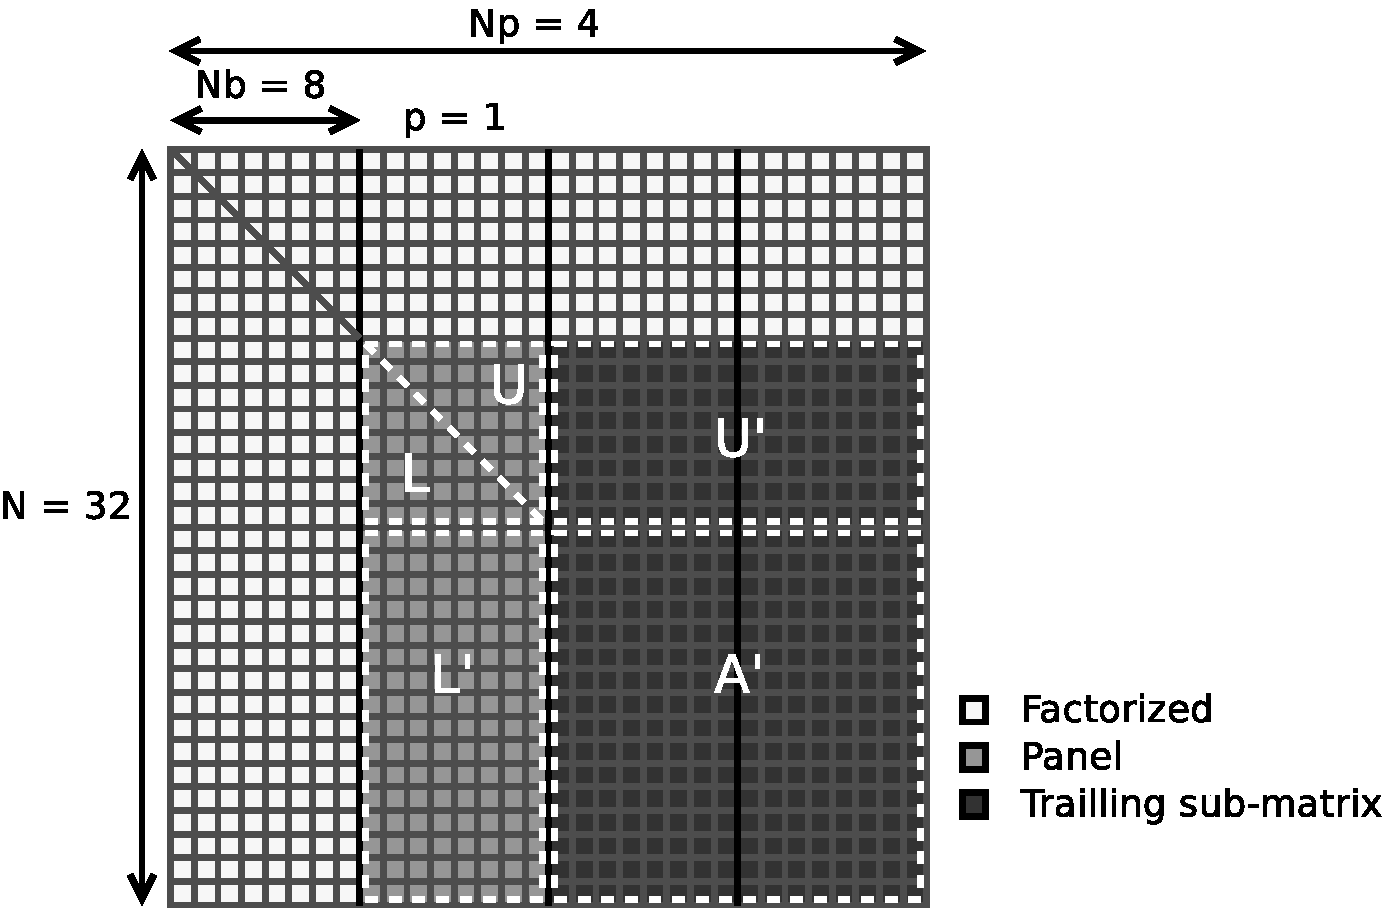
\includegraphics[width=0.8\textwidth]{figures/panel_matrix_bw.pdf}
\caption{LU decomposition at step $p$ on panel-blocked matrix \label{fig:matrix}}
\end{figure}

 
At each step $p$, the panel factorization is performed on the $p$th panel. Such a panel factorization consists in a loop of $n_b$ iterations. At each iteration $i$ ($p*n_b \leq i < (p+1)*n_b$), a search for the maximum of the $i$th column is performed, then its row is swapped with the $i$th row.
Then, a \textit{scal} operation is applied on the column $i$ and the trailing sub-panel is updated with an outer product - so called \textit{ger} according to the BLAS reference - (see Figure \ref{fig:panel}). The panel factorization produces an array of size $n_b$ containing the pivots selected, we note $ipiv$ this array. For each index $x$ of the array $ipiv$, the row $(p*n_b + x)$ will be swapped with the row $(ipiv[x])$.

\begin{figure}[!ht]
\centering
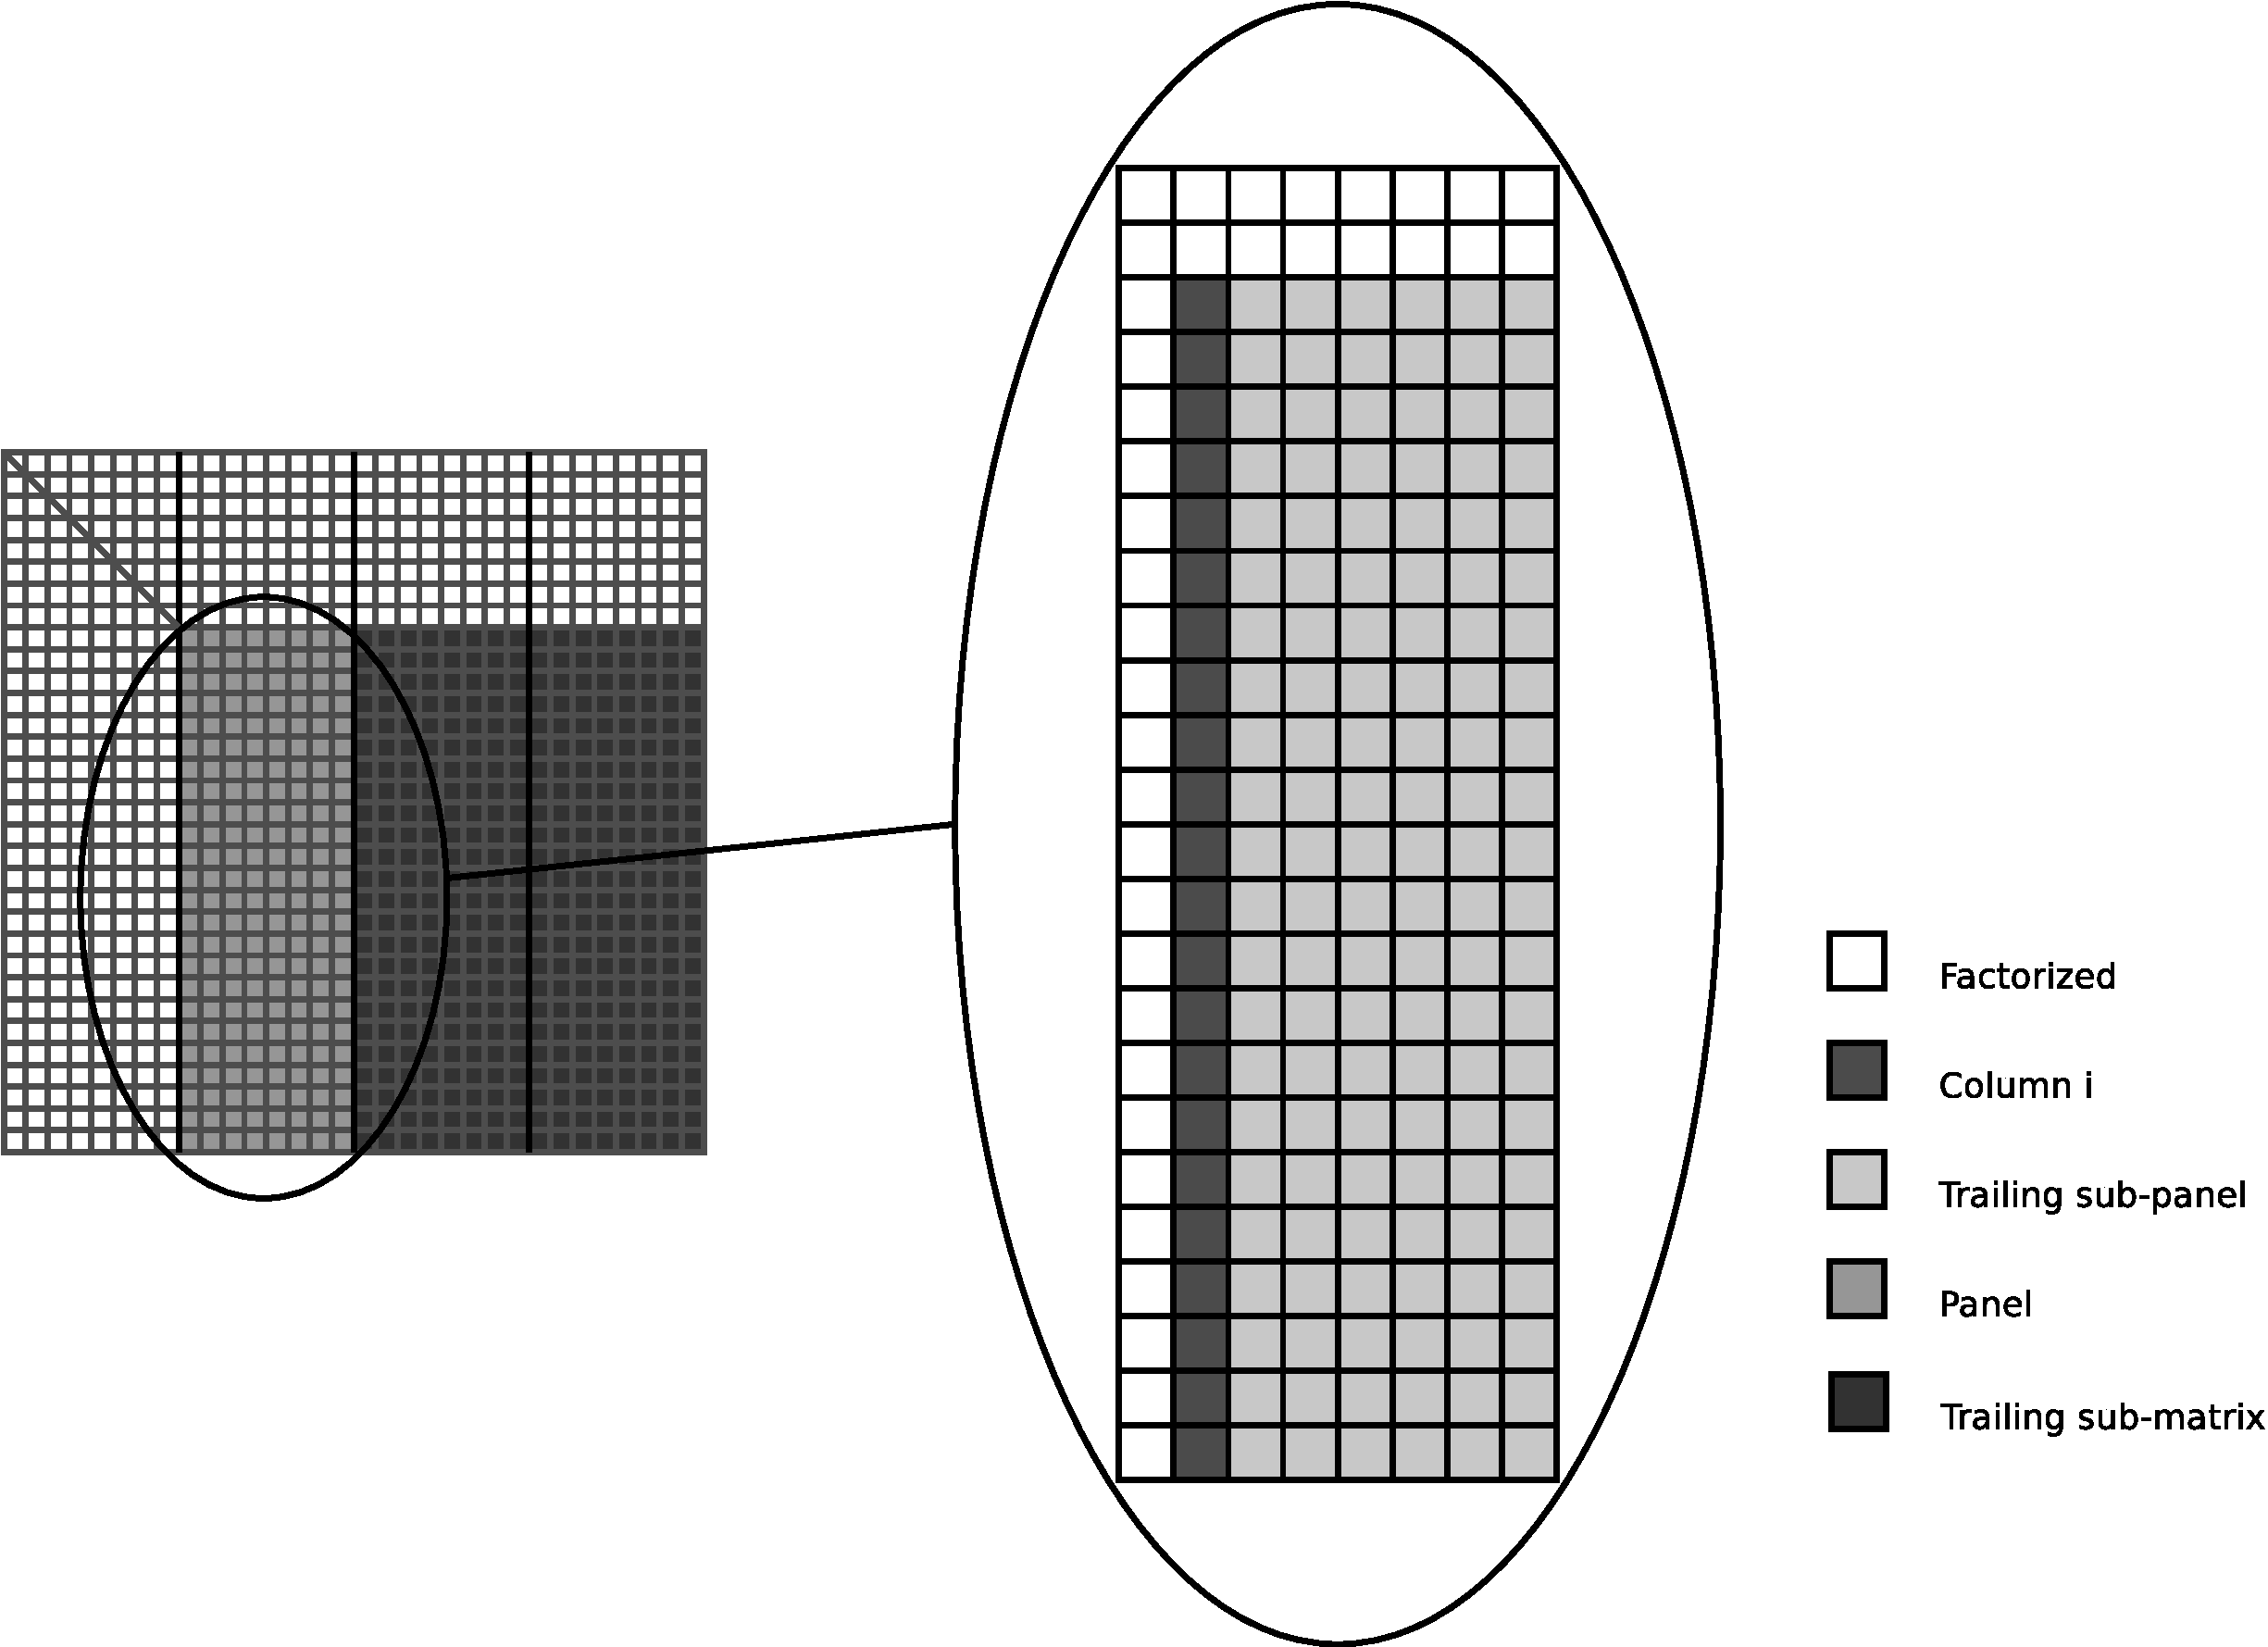
\includegraphics[width=0.8\textwidth]{figures/panel.pdf}
\caption{Second iteration of panel factorization (after swap)\label{fig:panel}}
\end{figure}

Once the $p$th panel is factorized, the subsequent trailing sub-matrix is updated. This update depend on the panel factorization. It takes as entry the pivot information and then applies the permutations on the whole trailing sub-matrix. Once the swap have been performed on the trailing sub-matrix, the $n_b$ block row corresponding to the eliminated rows (block $U$ in Figure \ref{fig:matrix}) is updated with \textit{trsm} operation. This block is then multiplied with a part of the panel (block $L$) and the resulting matrix is subtracted from the matrix $A'$ (this operation is performed with a \textit{gemm}).

\section{Task Flow LU Decomposition over Runtimes \label{task_flow_lu}}
Algorithm must be written as a task flow model in order to be executed over runtime systems (particularly on \dague). In the case of dense linear algebra, the algorithms have been redesigned to cope with this model. They are expressed in terms of tasks operating on fine grain squares sub-matrices, also called tiles \cite{conf/para/ButtariDKLLT06,ChanEtAl07b}. Figure \ref{fig:tiled_matrix} shows a matrix partitioned into tiles. In \cite{Buttari09}, the authors proposed a new pivoting strategy based on \cite{Quintana-Orti:2009:ULF} more suitable tile algorithms and achieved high performance by limiting the number of synchronizations, called \emph{incremental pivoting}. However, this algorithm has been proven numerically unstable \cite{journals/siammax/GrigoriDX11}. In order to achieve better stability, we choose to adapt the partial pivoting algorithm to the task flow model.

\begin{figure}[!ht]
\centering
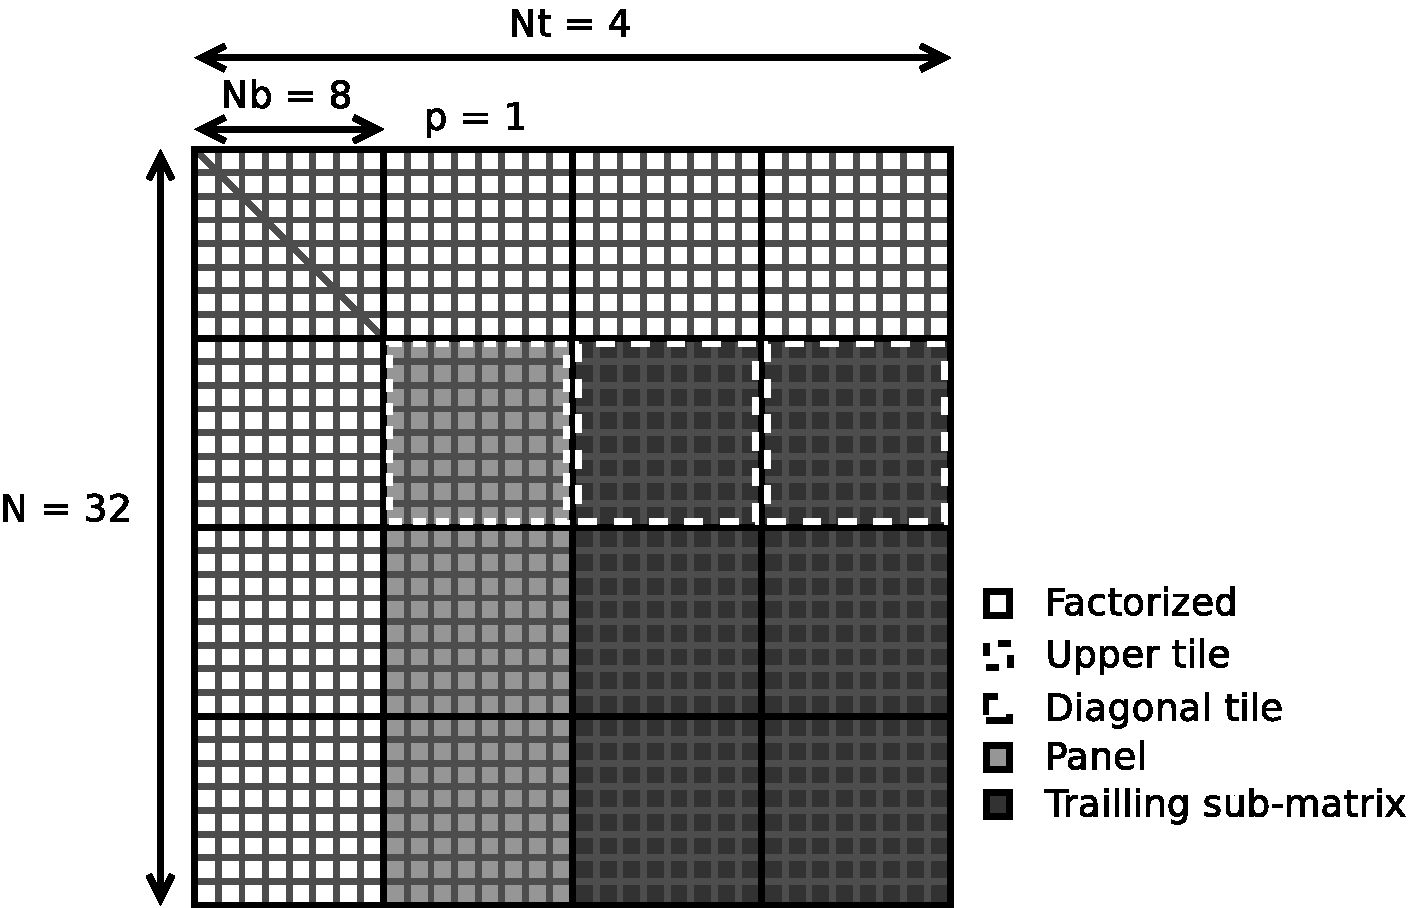
\includegraphics[width=0.8\textwidth]{figures/tiled_matrix.pdf}
\caption{LU decomposition at step $p$ on tiled matrix \label{fig:tiled_matrix}}
\end{figure}

To illustrate the complexity of implementing the algorithm, we consider the pivot search. This search occurs at each column factorization and lies on the critical path of the decomposition. Partial pivoting requires to select the maximum of the elements below the diagonal of the column. Then elements lie on $(n-k)/n_b$ different tiles which may be potentially mapped on a huge number numbers of cores in order to ensure state-of-the-art loud balancing techniques. The search induces a synchronization at each column which may overwhelm all potential benefits of tile algorithms and deliver too many tasks to be processed by the runtime.

Another issue - to show the complexity of implementing the partial pivoting over the task flow model - is the swapping operations of the update. In fact, after receiving the pivots array from the panel factorization, the upper tile has to send some rows to other tiles and receive back the substitute rows. If the swap is done rows by rows. The upper tile may exchange a row with another tile of the panel depending on the numerical values of the pivots. The task flow model can thus no longer be statically build in advance but has then to be dynamically composed. Figure \ref{fig:dynamic} represent a simplified task flow of the sending operation with an automaton. Each time the execution of an algorithm will depend on a value of a data, we will call this phenomenon a \emph{data dependency}. The algorithm which contain data dependencies will be called \emph{dynamic algorithm}. These algorithm may be represented by automatons or others conditional mathematical objects. Unfortunately, almost runtimes supports only static representation of task flow (DAG). Thus, the challenge is to represent a dynamic algorithm with a static representation covering the collection of possibilities. A solution may to create a DAG with a path where all concurrent tasks are sequential and move conditions of transitions to the kernel of the tasks. Figure \ref{fig:static} represent the same dynamic algorithm of Figure \ref{fig:dynamic} with a DAG, we can see that all the tasks are represented sequentially and that the conditions of the dependencies are integrated to the kernels. This transformation may increase tremendously the number of tasks and communications required to execute the algorithm. In the next sections we will present how we reduce the size of this static representation to perform the panel factorization and then update the trailing sub-matrix.

\begin{figure}[!ht]
\begin{minipage}[!ht]{.5\textwidth}
\centering
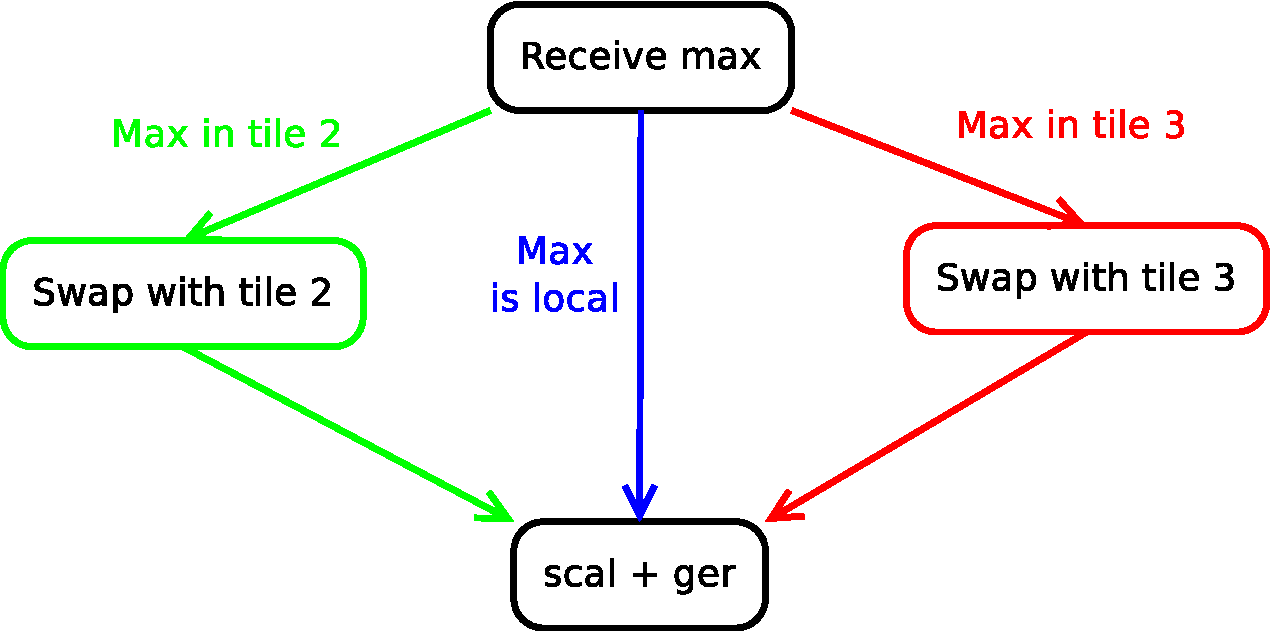
\includegraphics[height=3cm]{figures/dynamic.pdf}
\caption{Dynamic representation of task flow\label{fig:dynamic}}
\end{minipage} \hfill
\begin{minipage}[!ht]{.5\textwidth}
\centering
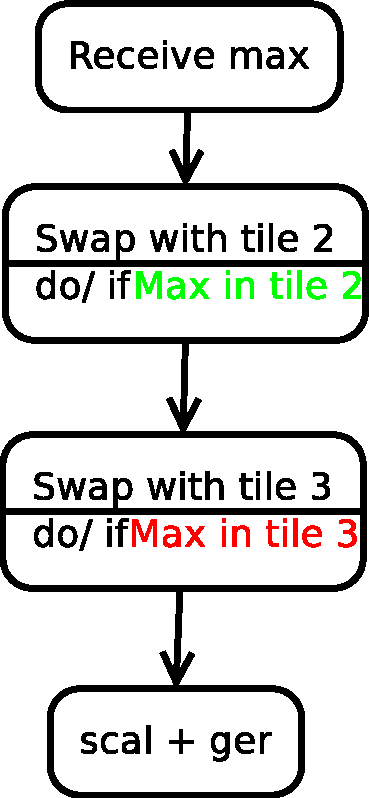
\includegraphics[height=4cm]{figures/static.pdf}
\caption{Static representation of task flow\label{fig:static}}
\end{minipage}
\end{figure}

\section{Platform models \label{platform}}
Fifteen years ago, a computer with only one single processor may be considered as computing platform and be included in the Top 500 ranking of super computers. Nowadays, computing platform have greatly evolved. Their architectures became more complex and varied. We propose here to distinguish them into four models.
\begin{itemize}
\item \textbf{Shared memory multi-cores architecture} is a computing platform consisting many cores and all have access to the same virtual memory.
\item \textbf{Distributed memory architecture} is composed of at least two node. Each node has its own cores and its physical memory. Cores of different nodes cannot access to the virtual memory of each other, and thus, must communicate to share data.
\item \textbf{Hierarchical architecture} is a distributed memory architecture where at least one node is a shared memory multi-cores architecture.
\item \textbf{Heterogeneous architecture} is a distributed memory architecture where at least one node is a GPU.
\end{itemize}

\chapter{Panel Factorization with Partial Pivoting}\label{panel}
In order to reduce the important number of tasks and communications, optimisations had to be applied at all levels of the algorithm. For that, we present in this section the evolution of the algorithm from the first natural version to the most optimized. As said in the section \ref{lu_algo}, the panel factorisation is a loop of $n_b$ iterations. At each iteration $k$, several operations are executed on the panel.
The first natural version is that the node which contain the diagonal node compare progressively its maximum with others tiles. Each time it find a better pivot, it saves it and uses it for next comparisons. After this operation, the diagonal tile broadcasts the initial diagonal row and the selected row owning the column maximum to all others tile in order that the concerned tile apply the swap, and every tile apply the \emph{scal} and \emph{ger} operations (Level 1 BLAS). Task flow \ref{fig:natural_task_flow} shows one iteration of the panel factorization on a panel of 6 tiles for distributed architecture.

\begin{taskflow}[!ht]
\centering
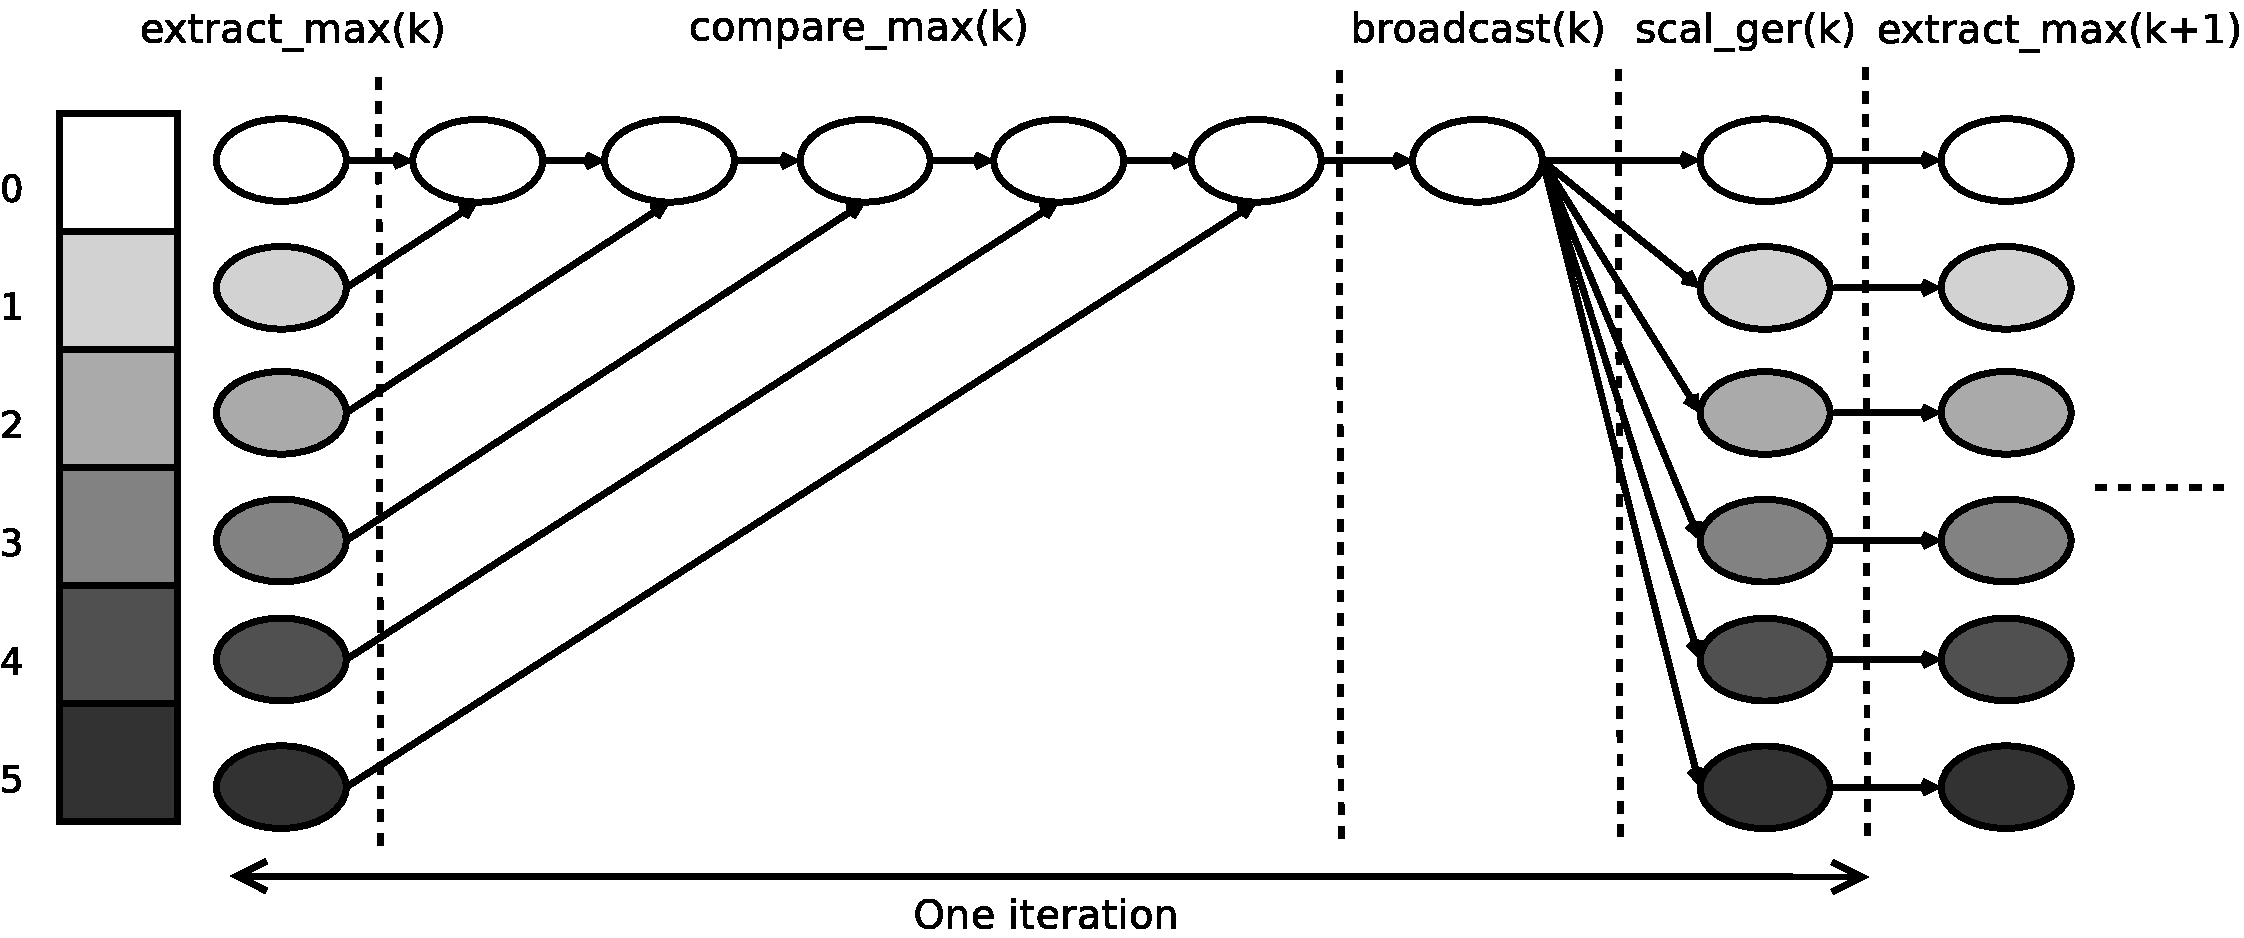
\includegraphics[width=0.8\textwidth]{figures/natural_tf_bw.pdf}
\caption{One iteration of panel factorization on distributed architecture \label{fig:natural_task_flow}}
\end{taskflow}

The first remark is that there is some communications which can be optimized. In fact, instead of using natural sequential comparison, it is possible to use a \emph{reduce} operation. It will allow to perform a faster election of the row consisting the maximum of the column. Therefore, because the broadcast is following the operation of comparison, we can merge the two operations into one single \textit{all\_reduce} operation.
We can also merge tasks of extraction and tasks of panel update. For that, the \emph{extract\_max} of step $k$ and \emph{scal\_ger} of step $k-1$ tasks can be done in one single task.

Concerning communications, \dague and other runtimes handle point-to-point communications and can manage some collective communications as broadcast or group communications. But, to perform more complex communications operations (reduce, gather\dots), we have to express them as a task flow. 
%This is due to the programme model. In fact, a point-to-point communications or a broadcast are just a set of arrows between nodes of the PTG. 
This is due to the fact that a complex communication had to associate a function to communications which not expressible with PTG. For the \emph{all\_reduce} operation, the task flow needed is based on the task flow of the Bruck's algorithm \cite{BruckEtAl97}.
In the natural version, we broadcast two rows (the initial diagonal row and the resulting maximum row). Thus, for the \emph{all\_reduce} operation, an array of two rows per node is needed, we will call it a workspace. The first one is filled at beginning by the diagonal tile with the initial diagonal row, and the second row is filled by all tiles with their maximum row. At each step of the \textit{all\_reduce} operation, task copy first row from the received workspace if it is not empty, and reduce the maximum row in the second row of their workspace. Thus, at the end of the \textit{all\_reduce} operation, all workspaces will be filled with the same values.
The resulting task flow is presented in Task flow \ref{fig:distributed_task_flow}.

\begin{taskflow}[!ht]
\centering
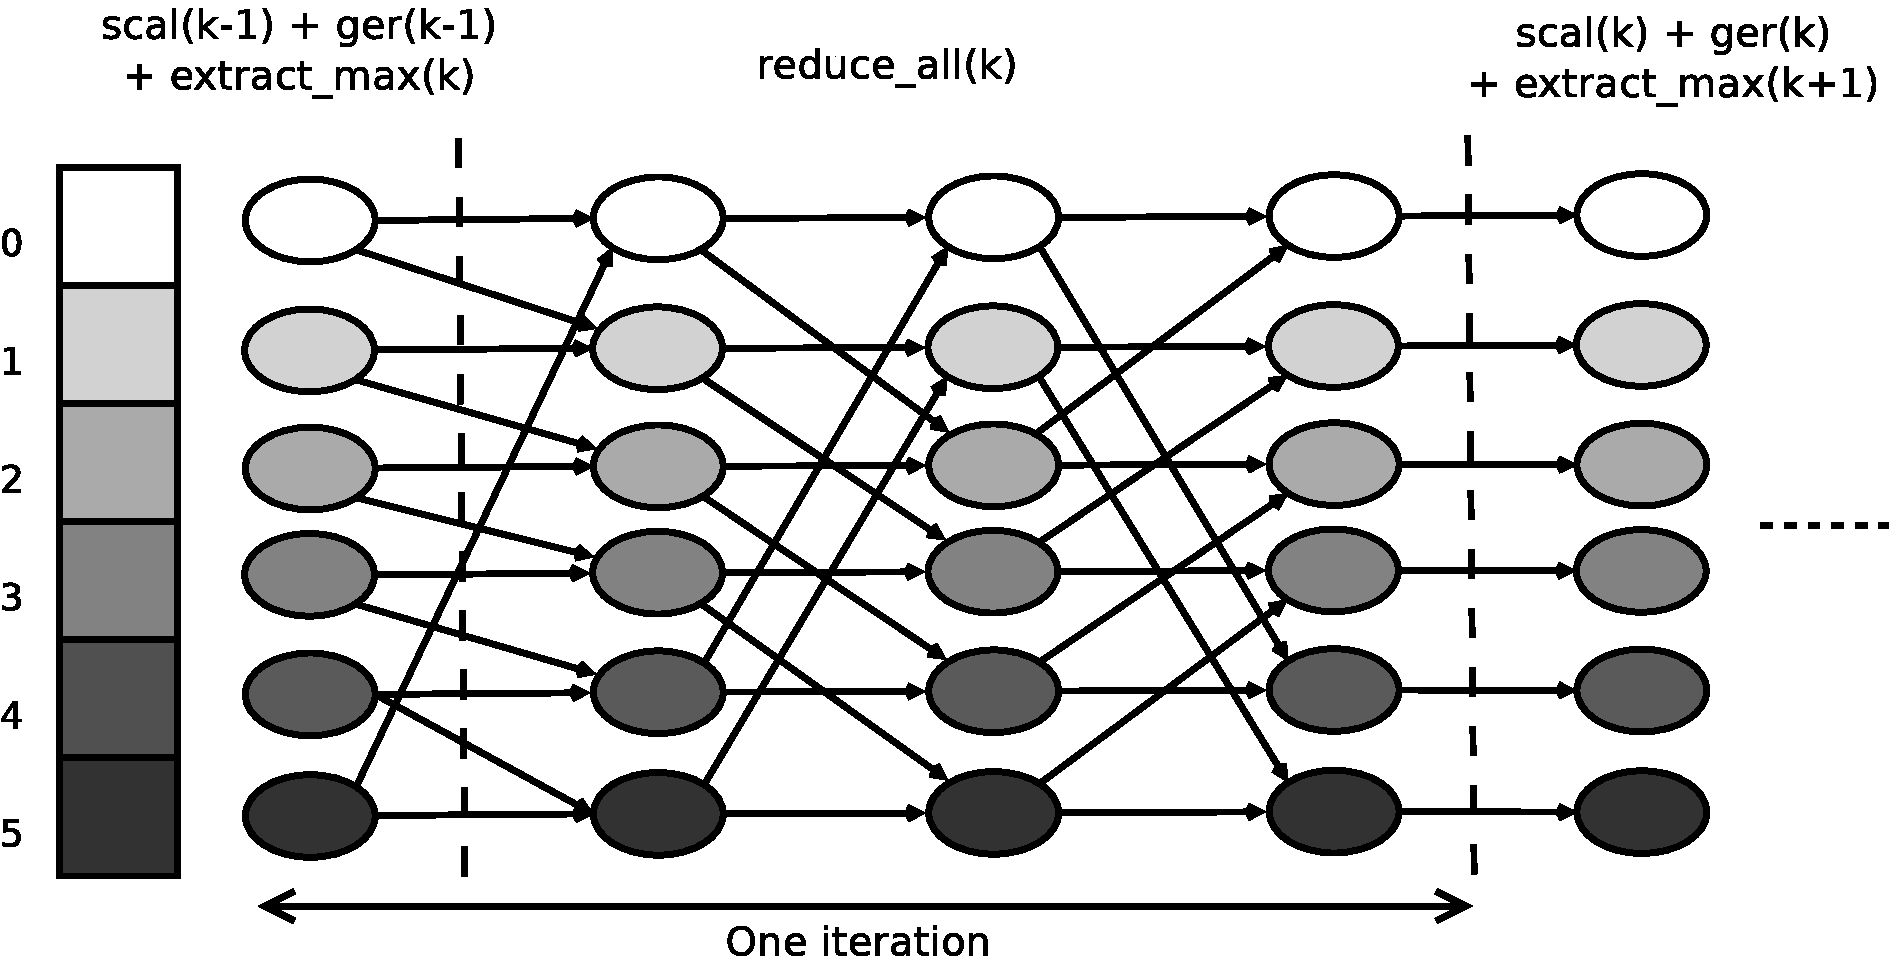
\includegraphics[width=0.6\textwidth]{figures/distributed_tf_bw.pdf}
\caption{One iteration of panel factorization on distributed architecture (combining reduce and broadcast communications)\label{fig:distributed_task_flow}}

\end{taskflow}

Nowadays, most distributed computers contain many cores at each node. To balance well the computations among the processors, a two-dimensional block-cyclic distribution is used to spread the data over the nodes\cite{DGW:SHPCC92}.
If we consider the fact that each node can be multi-core, the task flow \ref{fig:distributed_task_flow} can still be optimized. For that, the idea is to reduce first locally the maximum on the node and then, apply the \emph{all\_reduce} operation between the nodes. The \emph{reduce} operation is performed with a binary tree. Task flow \ref{fig:hybrid_task_flow} shows one iteration of panel factorization for hierarchical architecture. As for task flow \ref{fig:distributed_task_flow}, a similar workspace is used for \emph{all\_reduce} communications with one difference. The workspace contains four rows: two for the diagonal row and two for the maximum row. In fact, at each step of the panel factorization, only one of the two row is used depending on the step parity. This configuration is necessary to protect from the \emph{read after write} effect on the workspace  which is shared between all tiles of the same node.

\begin{taskflow}[!ht]
\centering
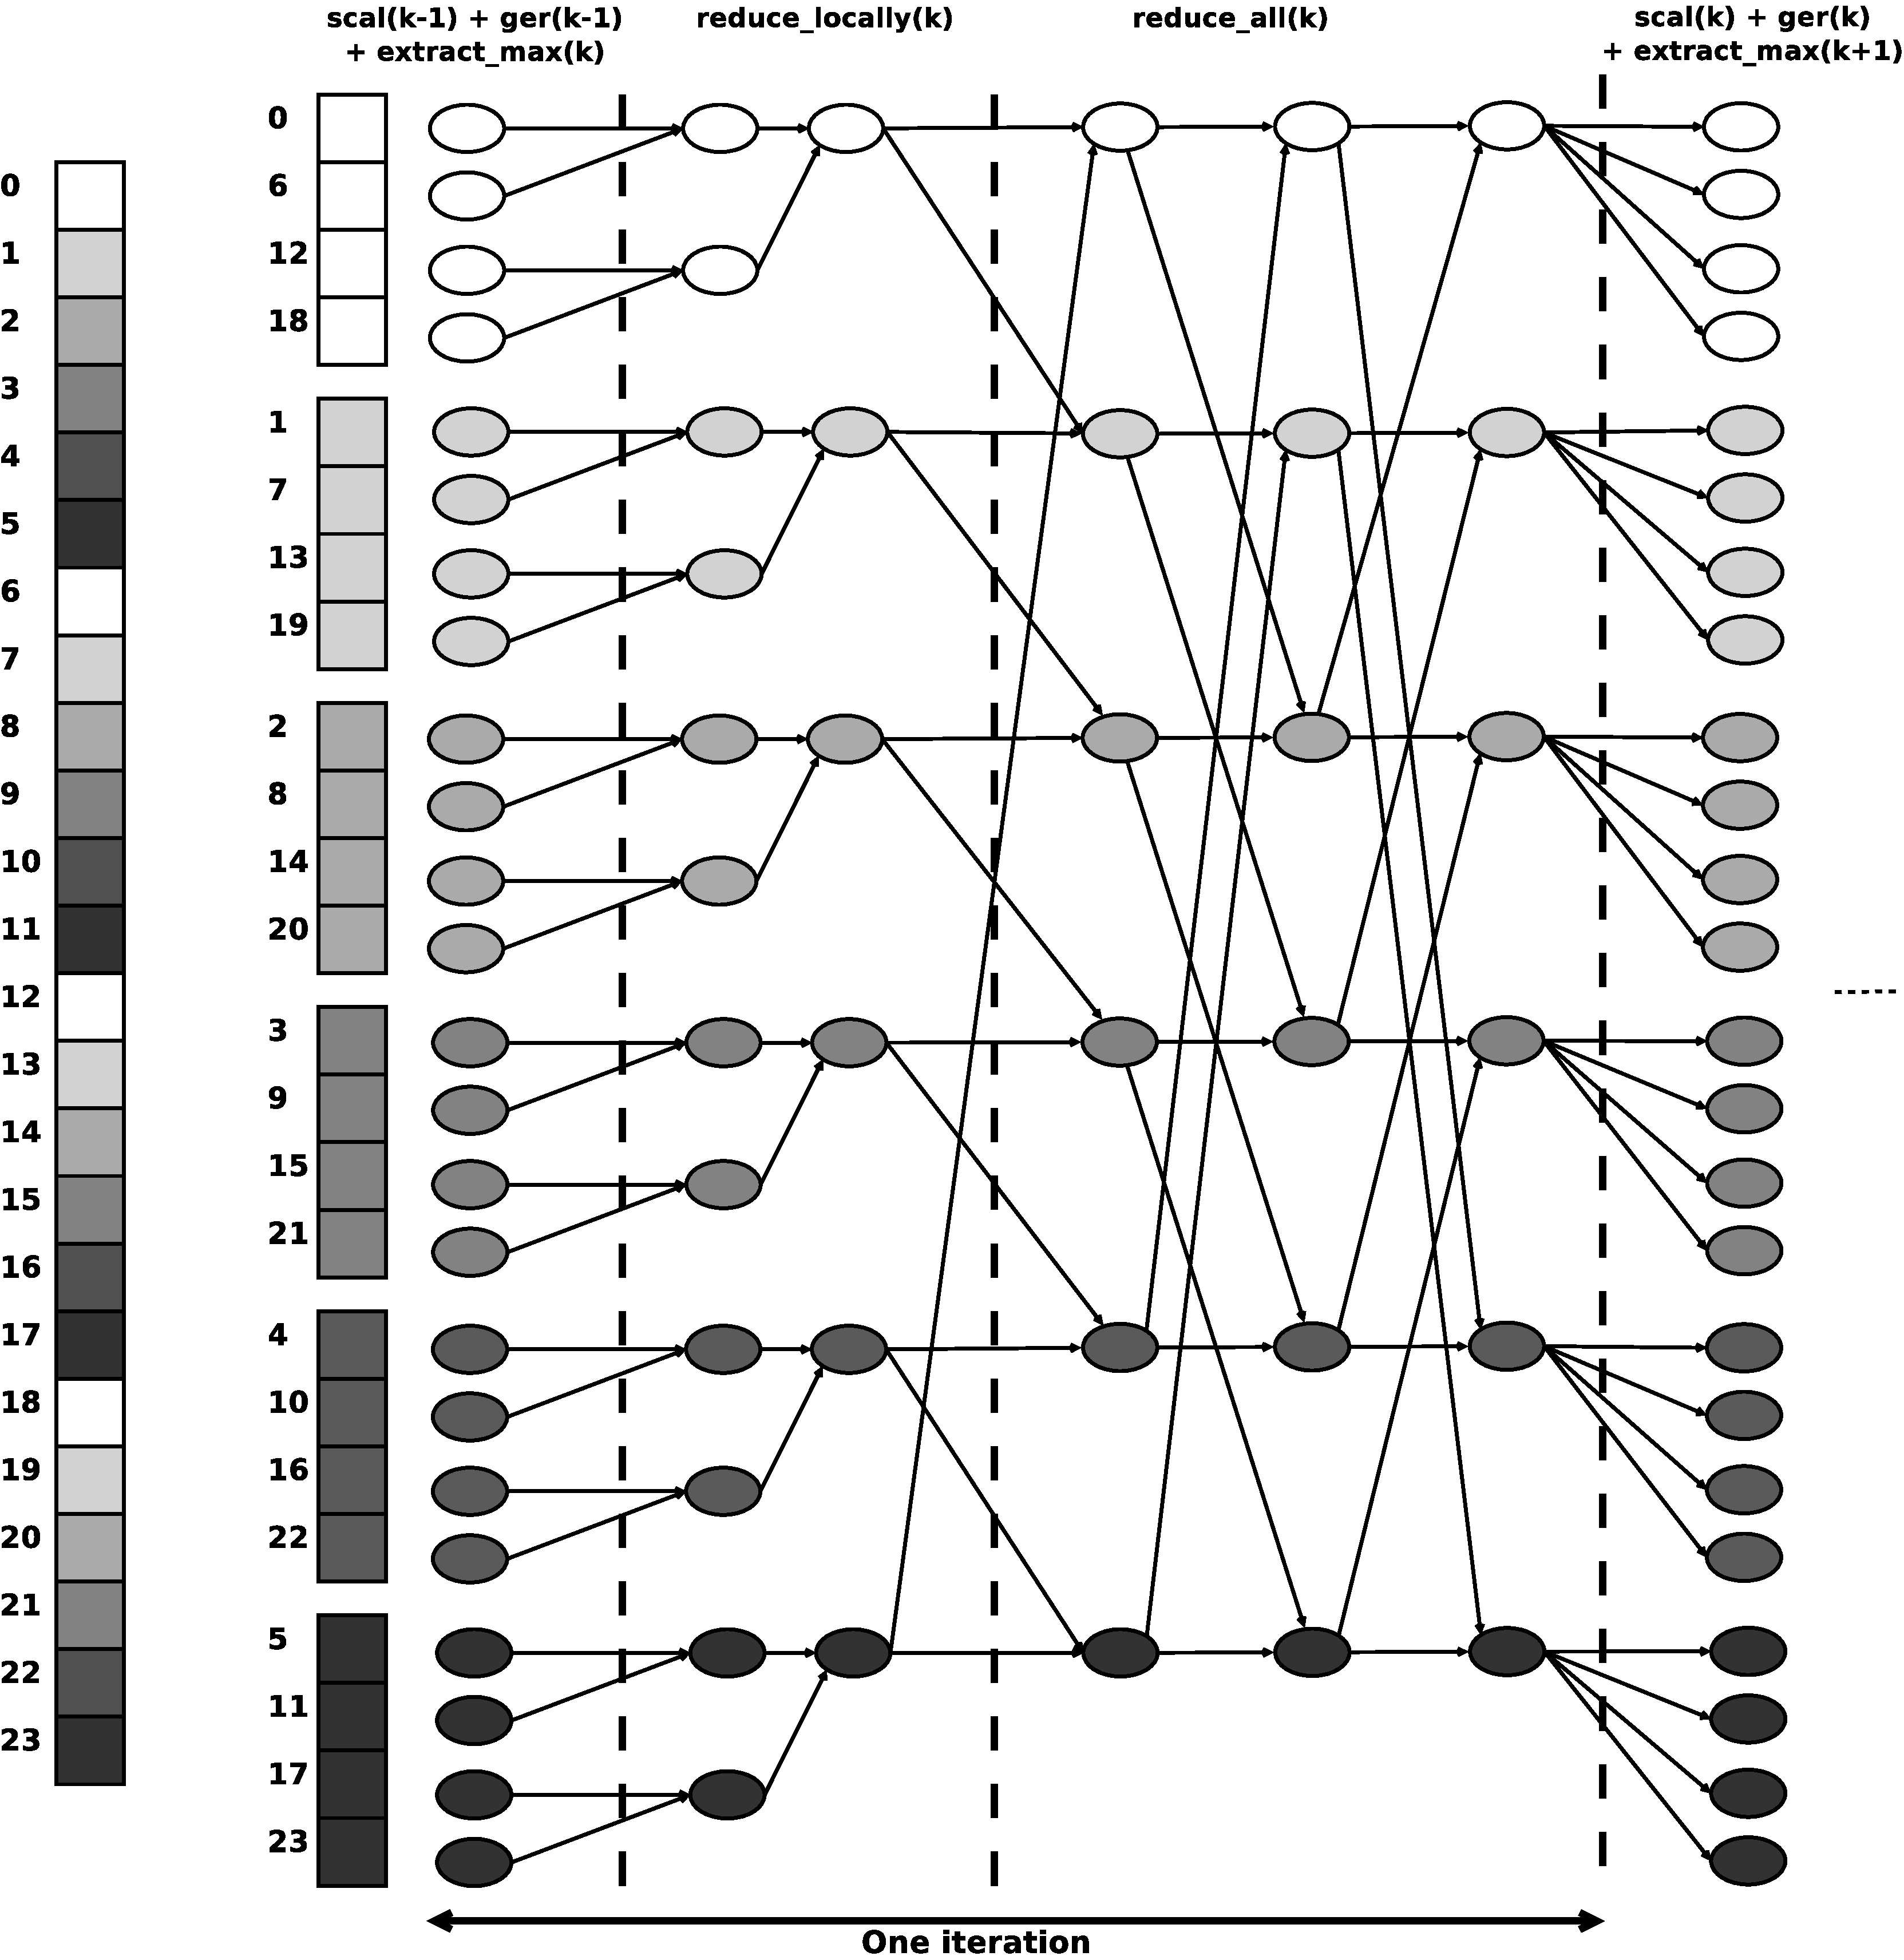
\includegraphics[width=0.7\textwidth]{figures/hybrid_tf_bw.pdf}
\caption{One iteration of panel factorization on hierarchical architecture \label{fig:hybrid_task_flow}}
\end{taskflow}
 
Whether in distributed, shared or hierarchical, the task flow showed in Task flows \ref{fig:natural_task_flow}, \ref{fig:distributed_task_flow} and \ref{fig:hybrid_task_flow} represent only one iteration of panel factorization. For the last iteration, an additional task is needed to finalize the panel factorization. In fact, this task perform the last \emph{scal} and \emph{ger} operations then release the dependencies to update the trailing sub-matrix.

Beside optimizations in task flow, we apply some optimization on kernel executed by tasks. In case of the task \textit{scal+ger+search\_max}, we use the notion of internal blocking. This optimization is the same applied from linpack to lapack library \cite{Anderson:1990:LPL}. Thanks to the internal blocking, we can use more Level 3 BLAS which increase the performance obtained. In fact, at each step of the panel factorization, instead applying ger on the whole trailing sub-panel, we apply it only on a block. After each $ib$ iterations, $ib$ being the internal blocking parameter, the rest of the trailing sub-panel is updated by the level 3 BLAS operations \textit{trsm} and \textit{gemm} (Figure \ref{fig:panel_ib}).

\begin{figure}[!ht]
\centering
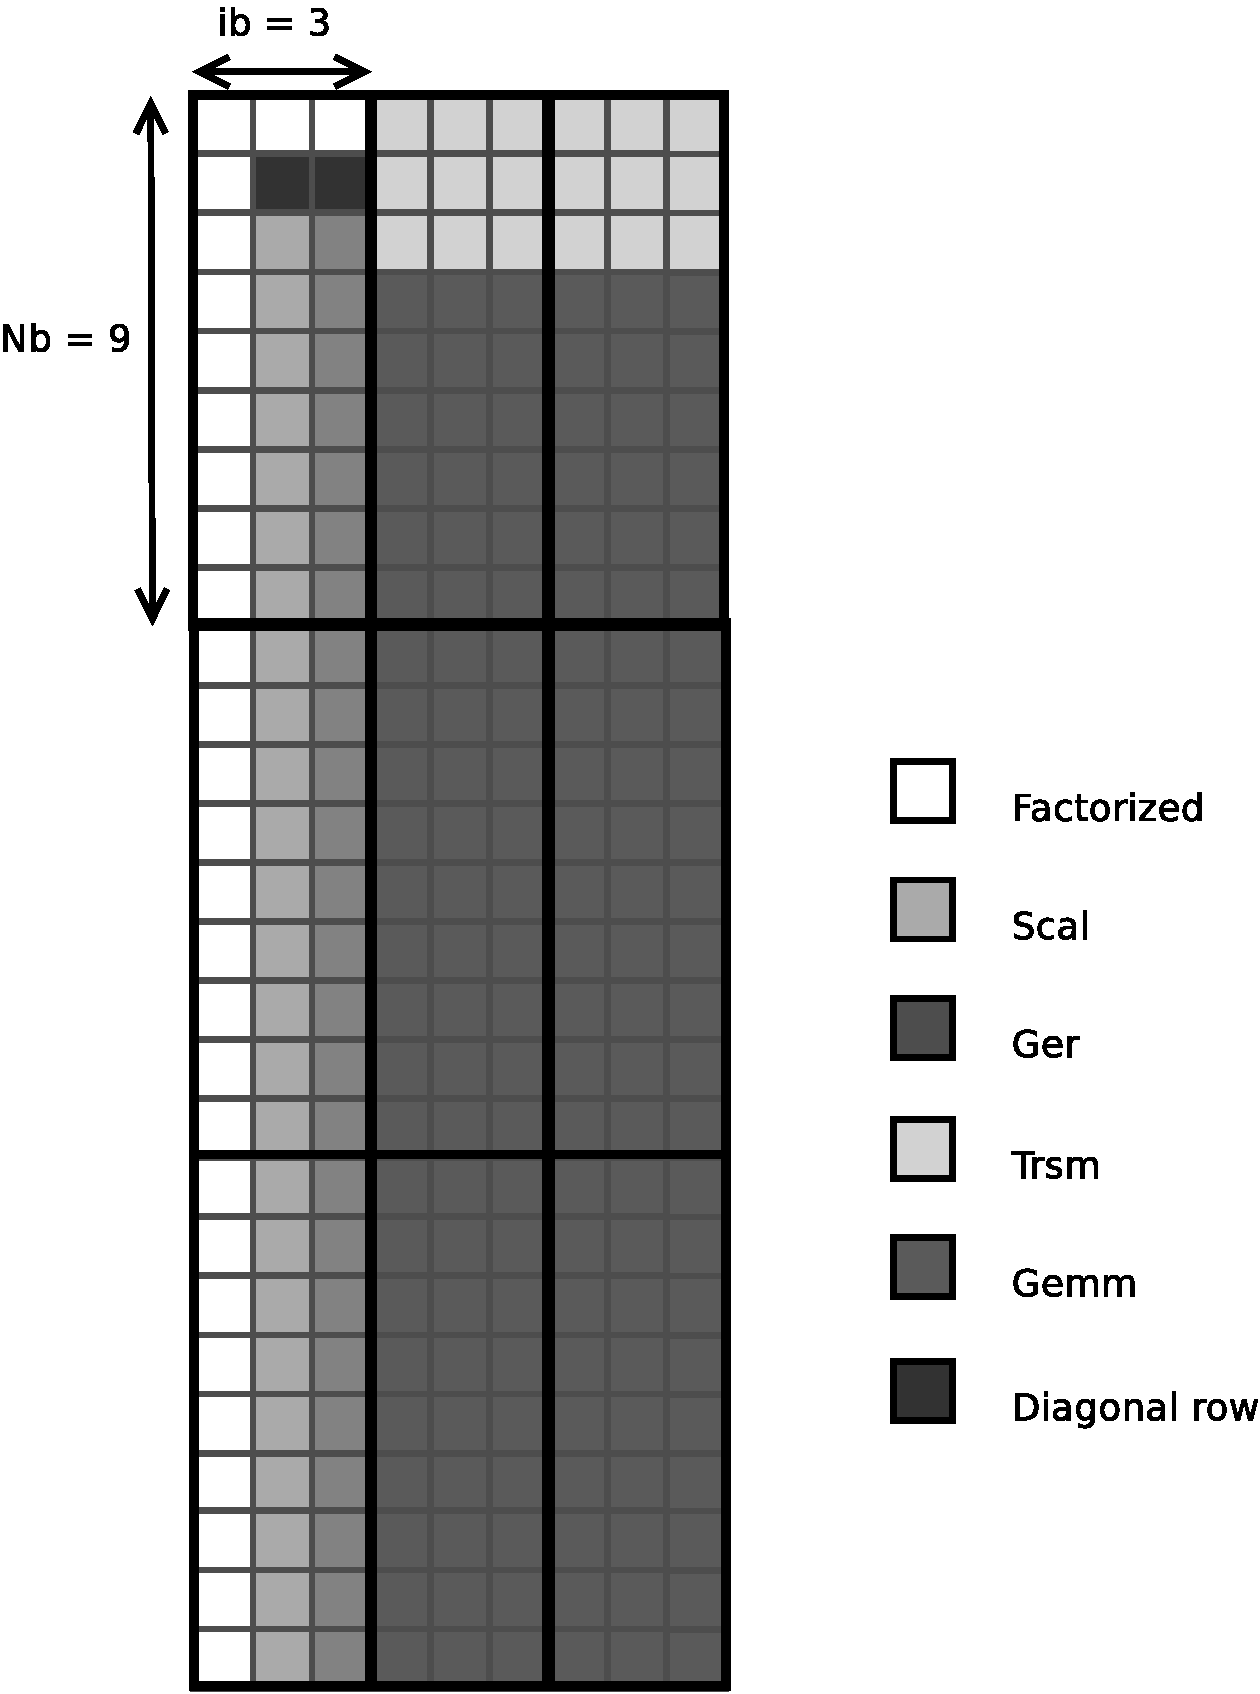
\includegraphics[height=8cm]{figures/panel_ib_bw.pdf}
\caption{Panel factorization with internal blocking\label{fig:panel_ib}}
\end{figure}


\chapter{Update engine for dynamic pivoting}\label{update}
After the panel factorization, the operation performed on the trailing sub-matrix is the update. The update takes the array of pivots produced by the panel factorization, swaps the rows and then apply \emph{trsm} and \emph{gemm} operations.

To perform one swap, the algorithm depend on the value of the pivots, this is what we call data dependency and so the algorithm is a dynamic algorithm (section \ref{task_flow_lu}). The solution to represent a dynamic algorithm with a static DAG of task flow is to make a path with all tasks. In practice, it means that all tiles must participate in swapping even if they are not concerned.
For that, each tile will have a workspace of two arrays: the first to store one row coming from the upper tile and the second to store one row going to the upper tile. Nodes will share between them the workspaces and fill them with the appropriate rows.
The \emph{all\_reduce} seems to be the right operation to use. The cost of a \emph{all\_reduce} operation is $log_2(n_t)$. Thus, the cost of all swaps of one panel is $n_b*log_2(n_t)$. This is very expensive relatively to the cost of SPMD model which is at most $2*n_b$.
Moreover, a the end of each \emph{all\_reduce} operation, only two nodes will really use the rows collected in their workspace (the upper tile and the tile which exchange with it).

A good idea is to perform all swaps at the same time. However, this is not possible with pivots. In fact, because the same row can be several time the maximum row, it is necessary to execute the pivots in the right order (from the first to the last). Figure \ref{fig:pivots} shows an example of a row which contains successively two time the maximum row, we can see that the row 1 goes down to the row 13 then comes back to the row 2. Thus, it forces us to perform the first pivots before the second.

\begin{figure}[!ht]
\begin{minipage}[!ht]{.4\textwidth}
\centering
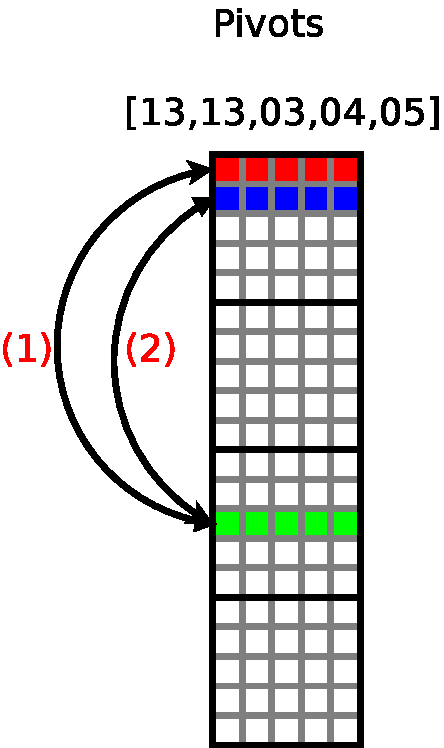
\includegraphics[height=5cm]{figures/pivots.pdf}
\caption{Row movements with pivots\label{fig:pivots}}
\end{minipage} \hfill
\begin{minipage}[!ht]{.4\textwidth}
\centering
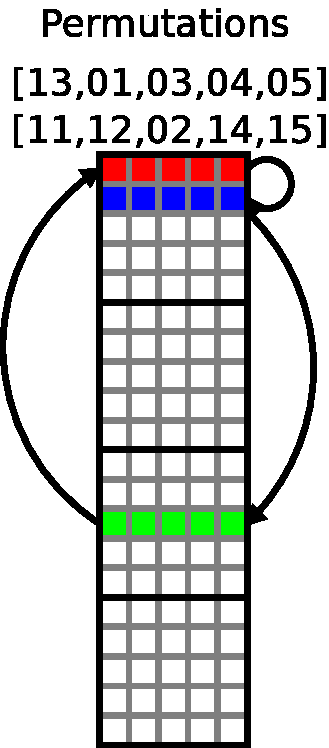
\includegraphics[height=5cm]{figures/permutations.pdf}
\caption{Row movements with permutations\label{fig:permutations}}
\end{minipage}
\end{figure}

To reduce high cost of all swaps, the key is to use another structure instead of pivots. For that, the permutations are the right solution. In fact, permutations can be represented by an array of size $n$ (we see after that it can be reduced). For each index $x$ of the array $perm$, the row $perm(x)$ will be moved in place of the row $x$. Thus, with permutations, we know from the beginning the final place of each row. 
Figure \ref{fig:permutations} shows the use of permutations instead of pivots which is showed in Figure \ref{fig:pivots}, we can see that the row 1 goes directly to the row 2 and does	 not move again.
Thanks to this structure, all the rows can be swapped in one single step and the cost will be just $log_2(n_t)$. 
We remark that at most $n_b$ rows go into and from the diagonal tile. Thus, the array of permutations may be limited to a size of $2*n_b$ elements, the first $nb$ elements will be used to store permutations and the second $nb$ elements will be used to store the inverse of permutations. Therefore, instead of using a workspace of two arrays, it is necessary to use two buffer - with size of tile - for communications: the first is a copy of the upper tile, it is shared from one node to the others. Each node will extract from the copy rows that it needs. We will call this operation \emph{swap from}. The second buffer is used to gather rows required by the upper tile. Each node creates its own buffer, fills it with rows intended to be stored in the upper tile and then participates with it in a \textit{gather} operation. This operation will be called \emph{swap into}. This solution allow us to perform the \emph{swap from} and the \emph{swap into} in parallel.

Task flow \ref{fig:distributed_update_task_flow} represents the swapping operation of update operation for distributed architecture. The bold arrows show some dependencies which add synchronizations to avoid \emph{read after write} effects. For example, the copy of the upper tile must be applied before its update.

\begin{taskflow}[!ht]
\centering
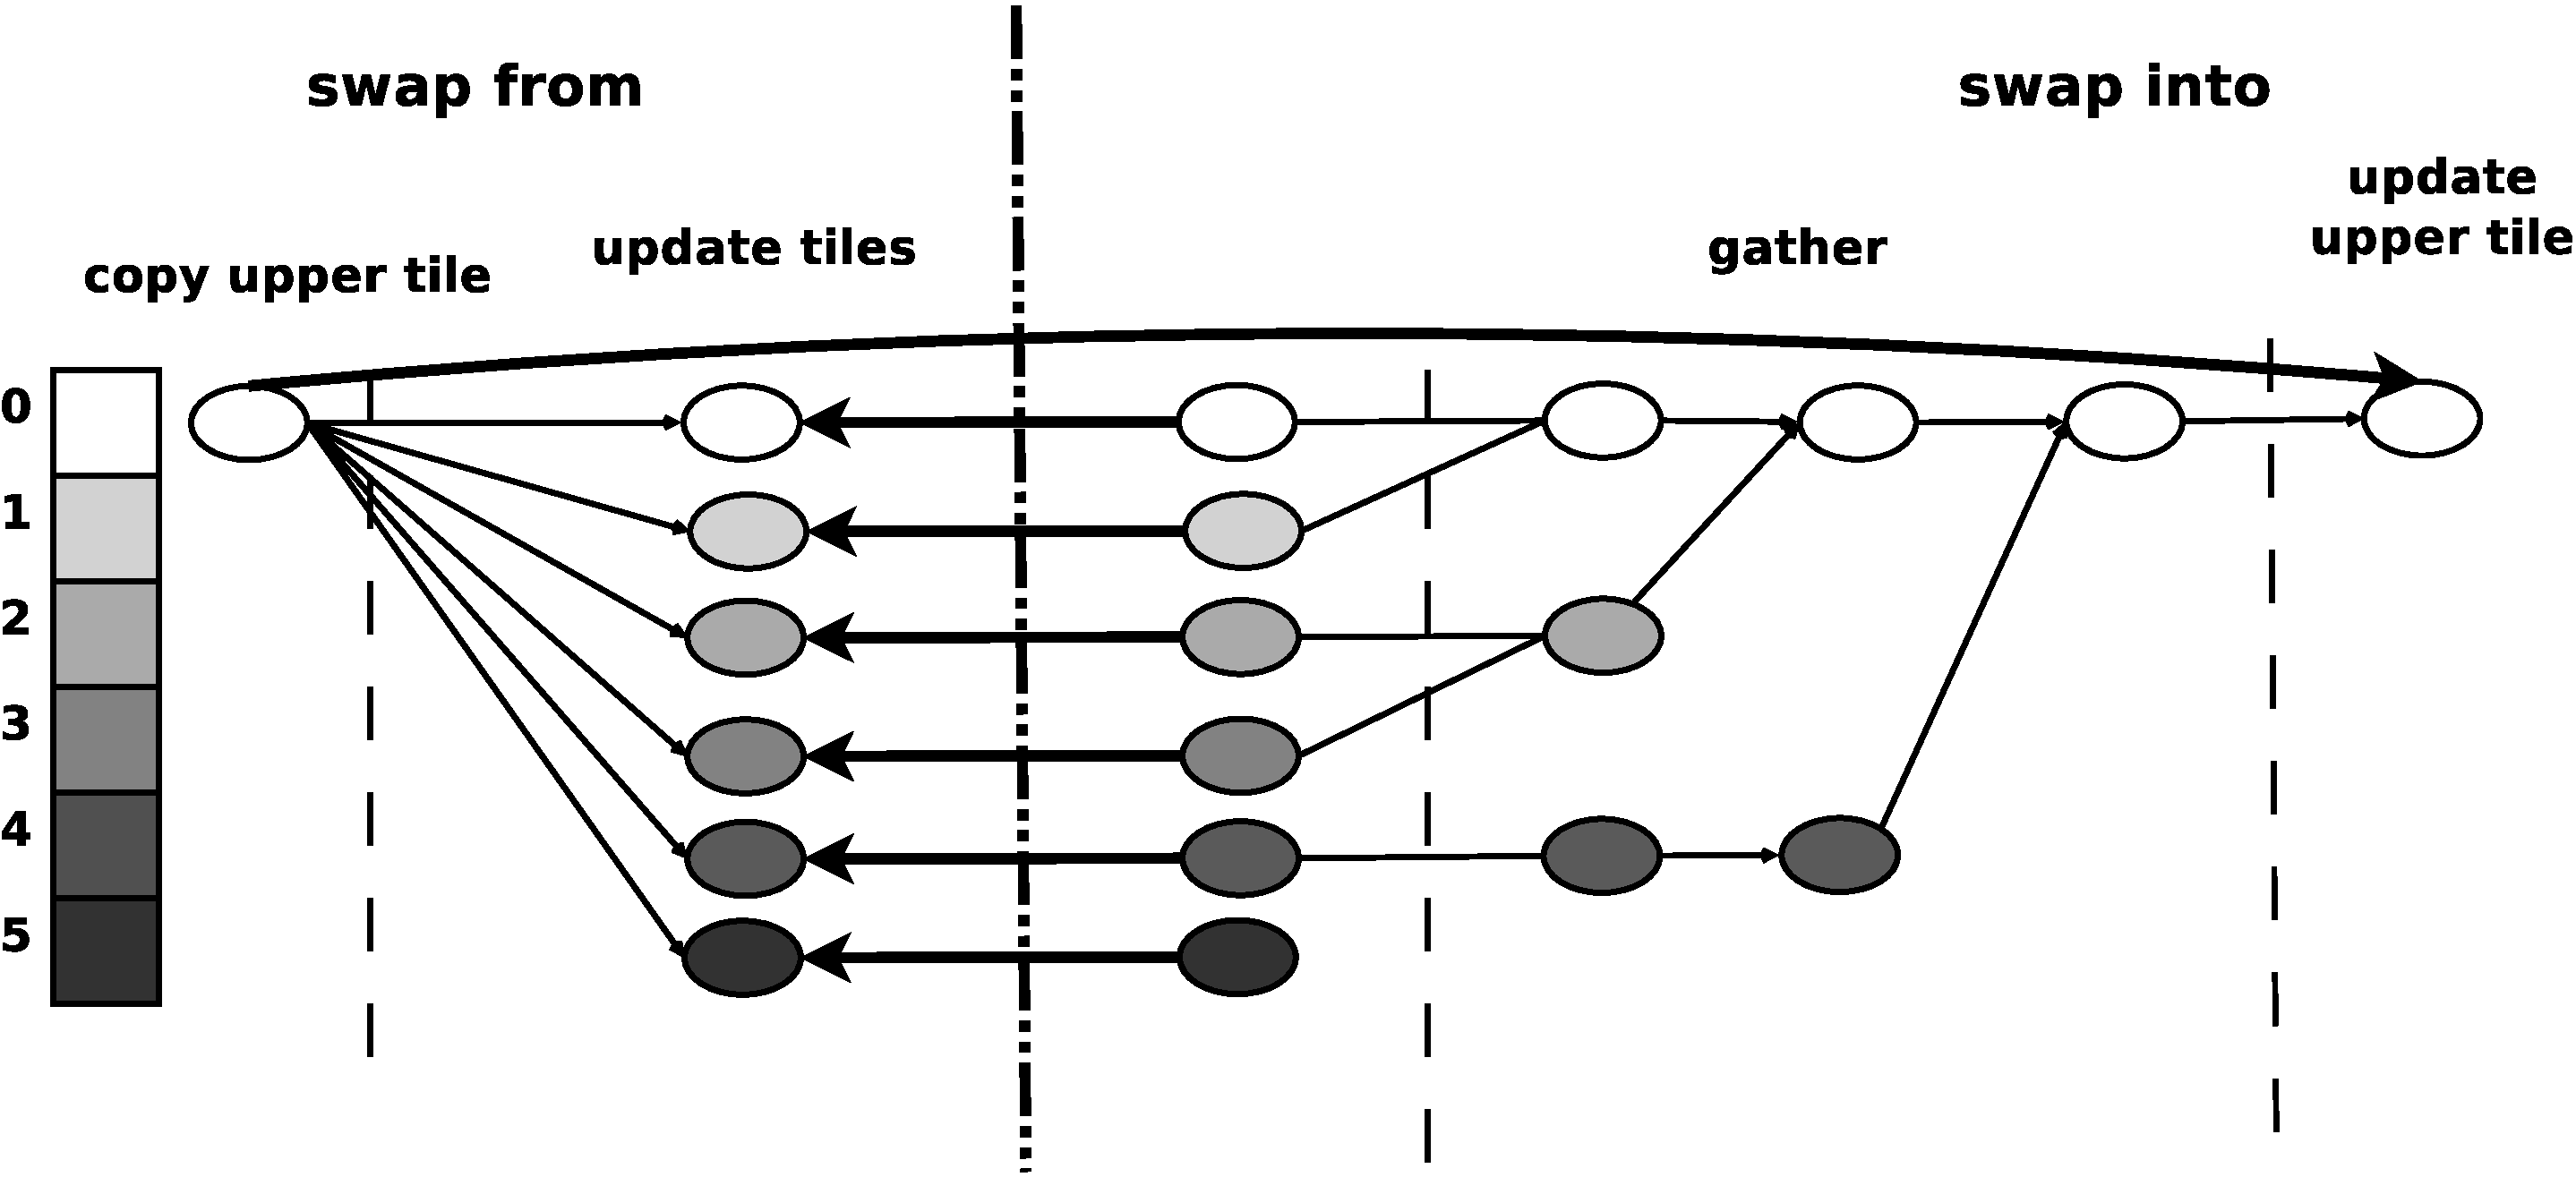
\includegraphics[width=0.8\textwidth]{figures/distributed_update_tf_bw.pdf}
\caption{Swapping operation of update on distributed architecture \label{fig:distributed_update_task_flow}}
\end{taskflow}

As for the panel factorization, we consider that nodes can be multi-core. In order to reduce global communication, each node shares its buffers over its local tiles before to send them to others nodes. Task flow \ref{fig:update_task_flow} shows the update operation for hierarchical architecture.

\begin{taskflow}[!ht]
\centering
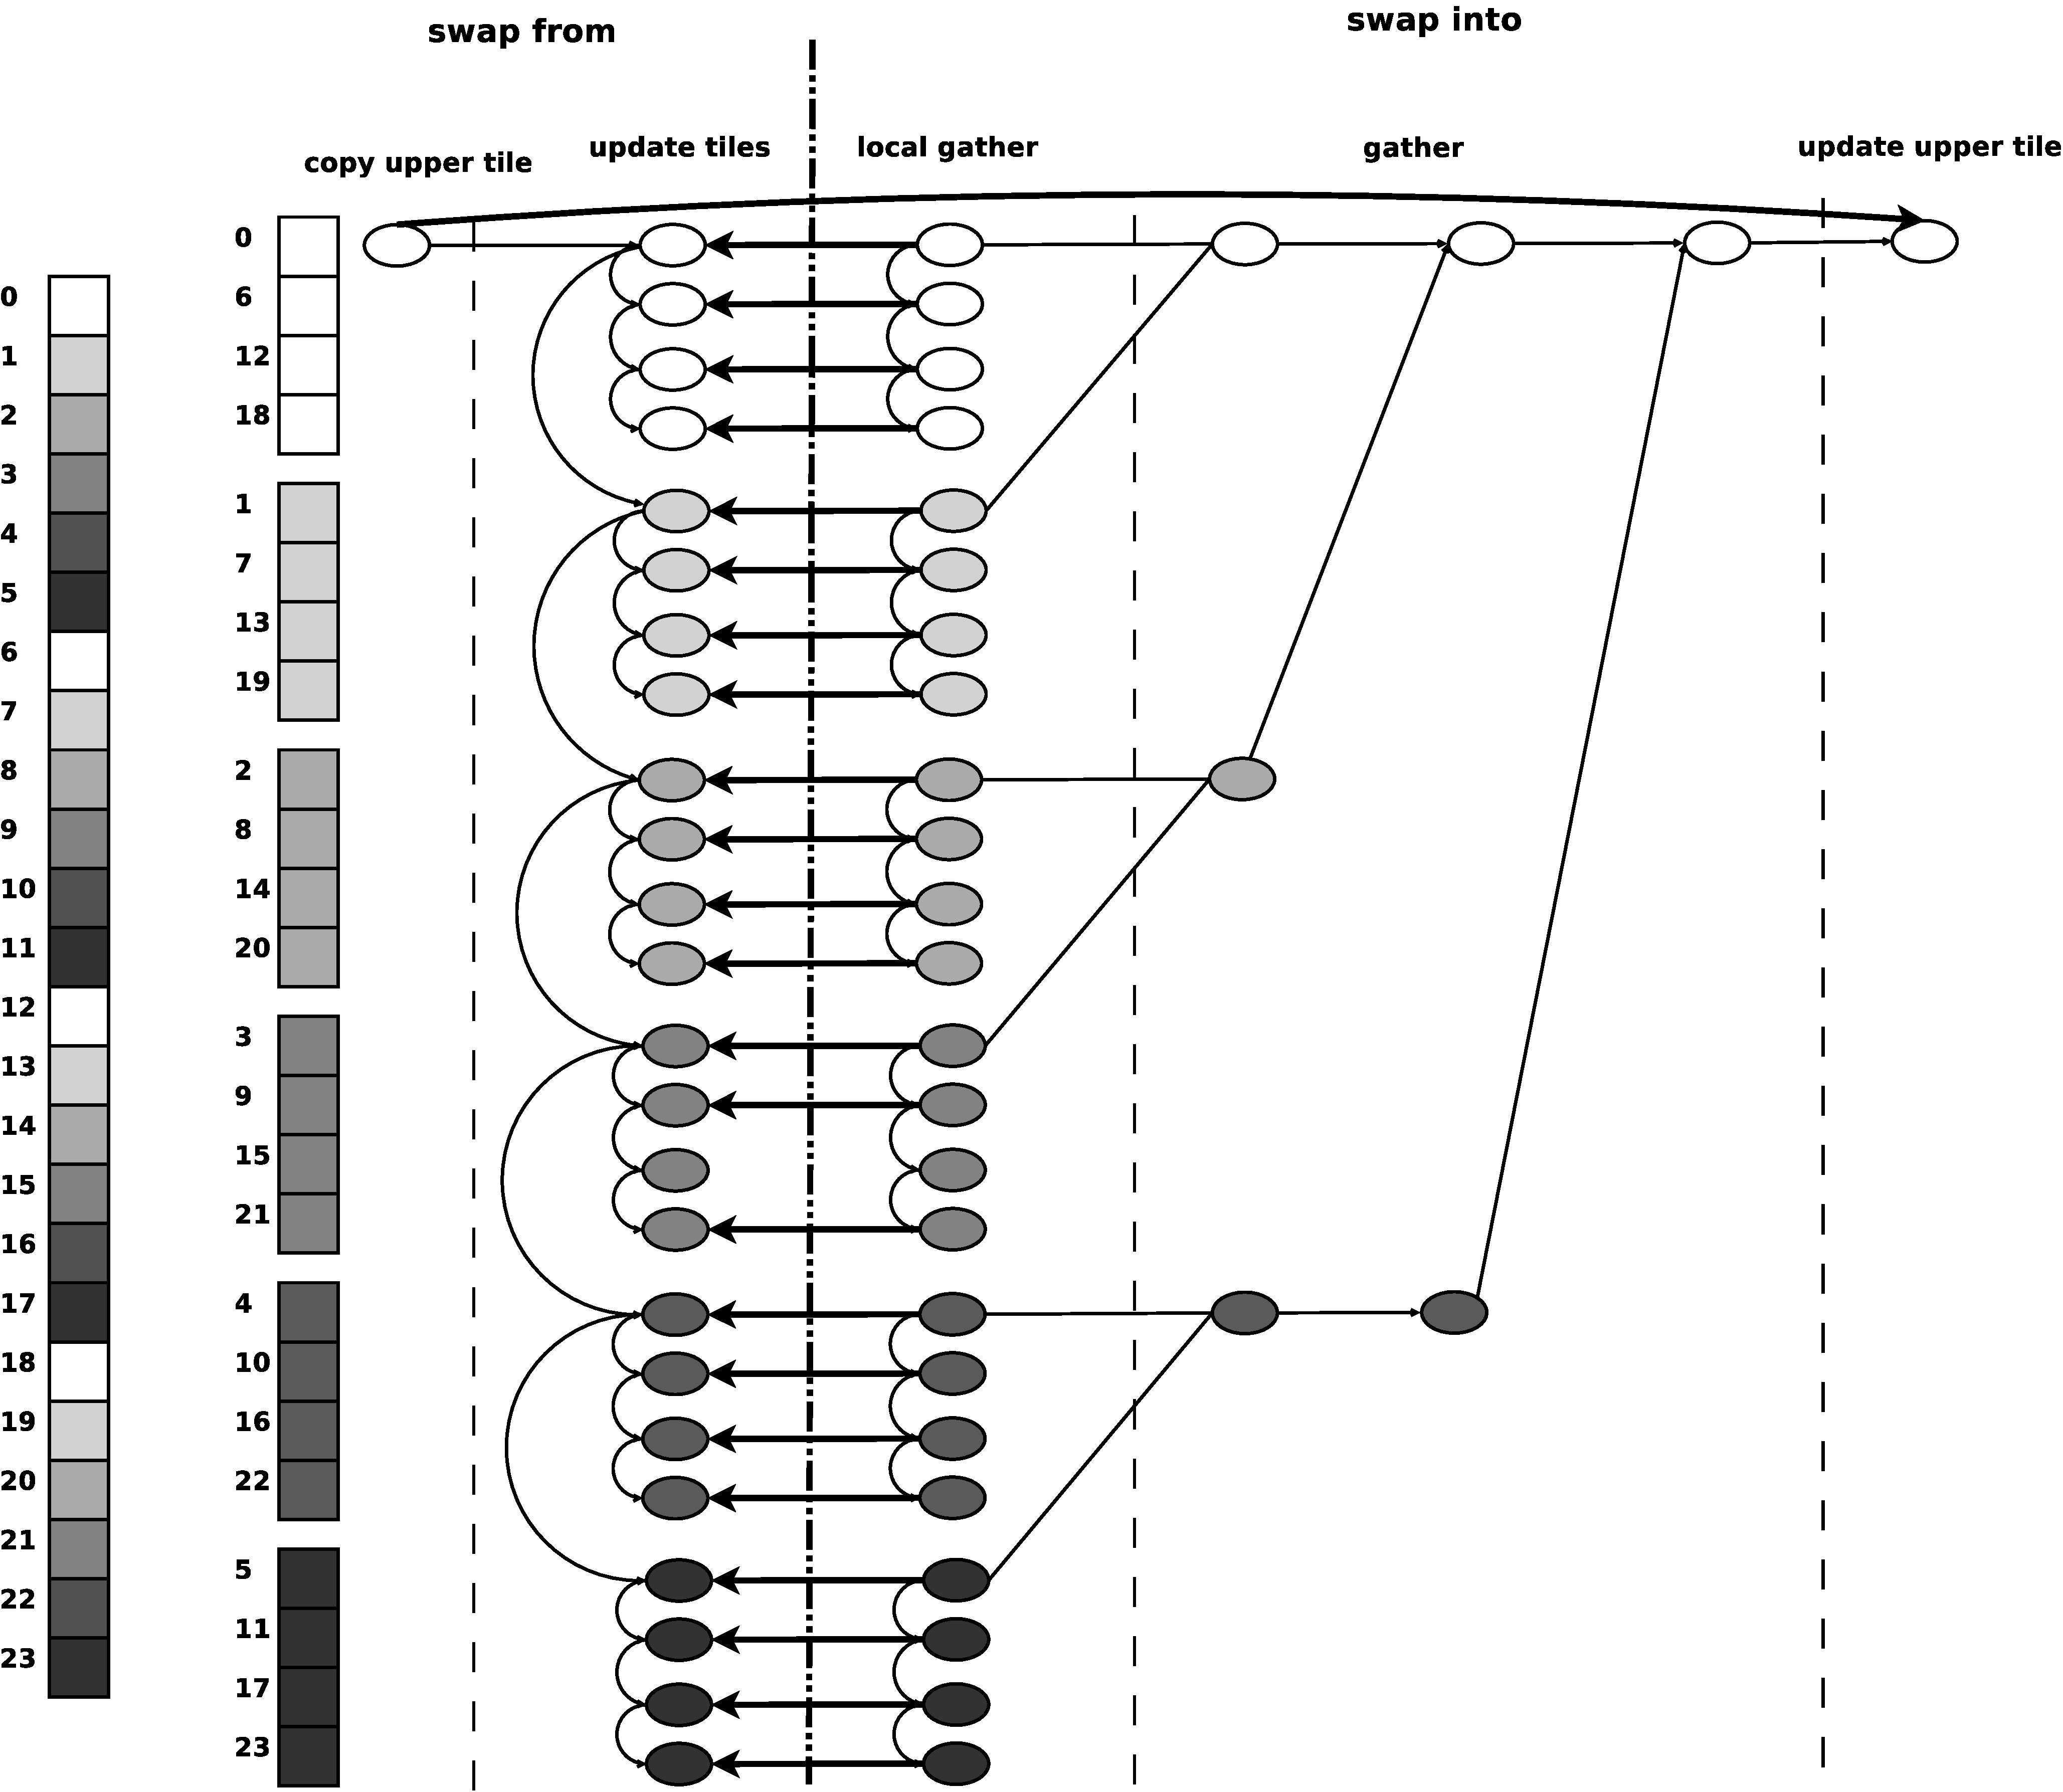
\includegraphics[width=0.8\textwidth]{figures/update_tf_bw.pdf}
\caption{Swapping operation of update on hierarchical architecture \label{fig:update_task_flow}}
\end{taskflow}

Moreover, this update algorithm implemented is a generic solution that it can execute update operation after any panel factorization which provide an array of pivots (incremental pivoting, CALU \dots).


\chapter{Experimental}\label{experimental}
In order to have an upper bound for the LU decomposition with partial pivoting, we also implemented an LU decomposition with static pivoting. It is similar to a partial pivoting but without swapping operation. It may be considered as a Cholesky's algorithm applied to the two sides of the matrix.

\dague and StarPU include already an implementation of LU decomposition with incremental pivoting. Thus, we compare them with the performances obtained of partial pivoting.

To complete the experiences, we also compare results with Scalapack performances.

\section{Exploiting hierarchical platform with PTG}
For this experience, we used \dague as PTG runner. The architecture used is and hierarchical platform. It consists of 128 cores distributed over 16 nodes and interconnected with an Infini Band. Thus, we implemented Task flow \ref{fig:hybrid_task_flow} for panel factorization and Task flow \ref{fig:update_task_flow} for swapping operations in update. The software used is Linux as operating system, \dague as runtime system and Intel Mkl library for Blas routines.

\begin{figure}
\centering
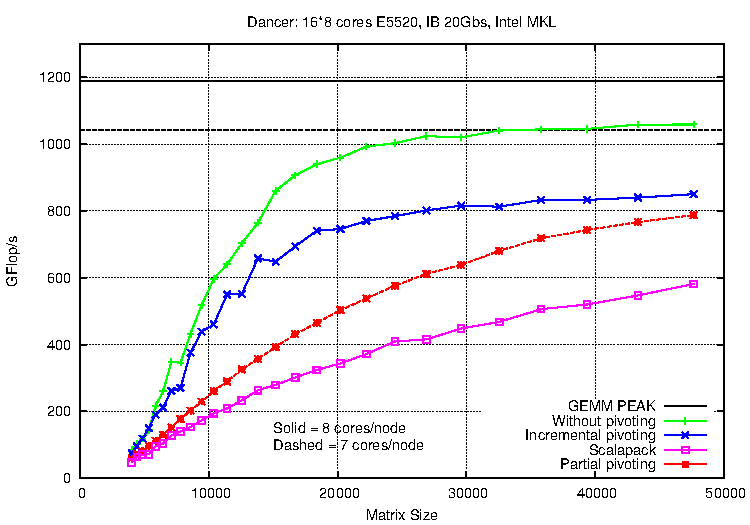
\includegraphics[width=0.8\textwidth]{figures/gepp.pdf}
\caption{Performance of LU decomposition with PTG\label{fig:pp}} 
\end{figure}

At the moment, the partial pivoting implemented was ran with only 7 cores by node for computation. The eighth core was completely dedicated to the communication. This was necessary to manage the high number of small communications on the panel. In the figure \ref{fig:pp}, it is showed two gemm peak, one using 8 core and the other only 7. The results obtained are satisfying. In fact,  the red curve - which is our implementation of LU decomposition over \dague - reaches 75\% of the gemm peak. Moreover, the performance of our LU decomposition are far better than Scalpack which is one of the most used mathematical library by the scientist community. 

%\section{Exploiting heterogeneous platform with sequential task flow}


%The distributed tests was applied on a machine of 16 nodes of 8 cores each, using an Infini Band network and the Intel MKL library.
%The first experiment applied was to take the static pivoting and plug on it the update engine implemented. Because all communications are done in every case, this test give the cost of the execution of the update engine. The result is showen in the figure \ref{fig:update}. The first remark is that the static pivoting is quickly approaching the gemm peak computer. This can be explained by the fact that all the getrf and trsm operations are recovered by gemm. The second curve is just a little below the first one. Thus, the update engine has a very small impact on the performances despite of its entire execution.  This is a very good result because first the update engine is generic and second its cost is very low.
%\begin{figure}
%\centering
%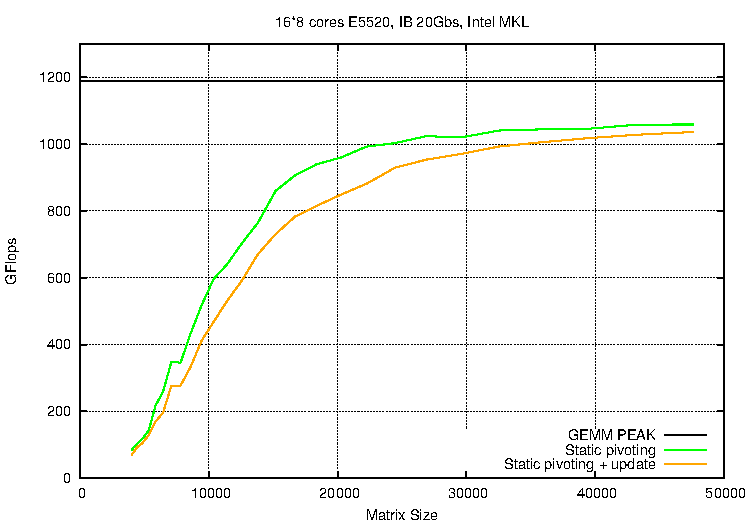
\includegraphics[width=0.8\textwidth]{figures/dgetrf_update_problem.pdf}
%\caption{Impact of the update engine on the performances\label{fig:update}} 
%\end{figure}
%The second experiment applied was the testing of the LU decomposition with partial pivoting implemented. It was compared to the incremental pivoting and the Scalapack implementation. At the moment, the partial pivoting implemented was runned with only 7 cores by node for computation. The eighth core was completly dedicated to the communication. This was necesary to manage the high number of small communications on the panel. In the figure \ref{fig:pp}, it is showed two gemm peak, one using 8 core and the other only 7.
%\begin{figure}
%\centering
%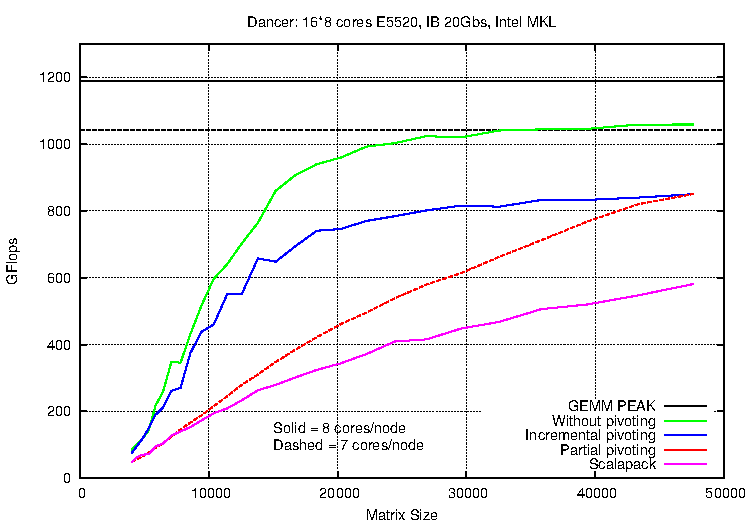
\includegraphics[width=0.8\textwidth]{figures/partial_pivoting_problem.pdf}
%\caption{Impact of the update engine on the performances\label{fig:pp}} 
%\end{figure}


\chapter*{Conclusion}\label{conclusion}
LU decomposition with partial pivoting is a dynamic algorithm with its data dependencies in the swapping operation for the update. Despite this difficulty, we managed to implement a task flow LU decomposition with PTG and obtained hopeful performances.

We try now to optimize the \dague runtime system to better manage the small communications messages, in order to take full advantage of all cores of nodes. 
Thanks to this representation of the algorithm, we hope to create an algorithm that will fully exploit heterogeneous architectures by offloading GEMM to accelerators as GPUs or Intel MIC on distributed architectures. Nowadays, GPU implementations of the LU partial pivoting are doing the ScaLAPACK sequential execution of the algorithm and offload the GEMM on the GPU, or are able to fully exploit a single heterogeneous node by using block-column distribution. This would be a disaster in the load balance on distributed architectures where a 2D block-cyclic distribution is require to decrease the volume of communication and average out the load over the multiple nodes. 
%We will be able to have one of the most efficient LU decomposition implementation. Beside its use for resolving system of linear equations, it will be possible to create a new benchmark to analyse computers performances.

In parallel, we implemented another task flow LU decomposition on StarPU. In fact, StarPU runtime allow to implement dynamic algorithm  thanks to its task insertion system. Moreover, it allow to make \emph{reduce} operation which enable to select the best pivot without using tree implementation. We will be able to compare results to PTG in general and \dague particularly.

\bibliographystyle{splncs}
\bibliography{report}

\end{document}

